% Compilar a .pdf con LaTeX (pdflatex)
% Es necesario instalar Beamer 
%

\documentclass{beamer}
\usepackage{moreverb} 
\usepackage{listings}
\usepackage{mflogo}
% imprimir
% \documentclass[handout]{beamer} 
% \usepackage{pgfpages}
% \pgfpagesuselayout{4 on 1}[a4paper,landscape,border shrink=5mm]

\mode<presentation> {
  \usetheme{Warsaw}
%  \setbeamercovered{transparent}
  \setbeamercovered{invisible}
}

\usebackgroundtemplate{
\includegraphics[width=\paperwidth]{format/libresoft-bg.png}}
% \usepackage[spanish]{babel}
\usepackage[utf8]{inputenc}
\usepackage{graphics}
\usepackage{amssymb} % Simbolos matematicos

%% Metadatos del PDF.
\hypersetup{  
  pdftitle={Legal Aspects},
  pdfauthor={Miguel Vidal},
  pdfcreator={GSyC/Libresoft},
  pdfproducer=PDFLaTeX,
  pdfsubject={Master on Free Software},
}
%%

\defbeamertemplate*{footline}{shadow theme}
{%
  \leavevmode%
  \hbox{\begin{beamercolorbox}[wd=.5\paperwidth,ht=2.5ex,dp=1.125ex,leftskip=.3cm plus1fil,rightskip=.3cm]{author in head/foot}%
    \usebeamerfont{author in head/foot}\insertframenumber\,/\,\inserttotalframenumber\hfill
\includegraphics[scale=0.40]{format/cc-by-80x15.png} \hspace{0.1cm}\insertshortauthor 
% \usebeamerfont{author in head/foot} 
\includegraphics[width=0.7cm]{format/cc-by.png} \hfill\insertshortauthor
  \end{beamercolorbox}%
  \begin{beamercolorbox}[wd=.5\paperwidth,ht=2.5ex,dp=1.125ex,leftskip=.3cm,rightskip=.3cm plus1fil]{title in head/foot}%
    \usebeamerfont{title in head/foot}\insertshorttitle%
  \end{beamercolorbox}}%
  \vskip0pt%
}

\begin{document}

\title{Legal Aspects}
\subtitle{Master on Libre Software (URJC)}
\institute{\texttt{http://gsyc.urjc.es/\~{}mvidal} \\ Twitter: \texttt{@mvidallopez}}
\author{Miguel Vidal} 
%\date{\today}
\date{November, 2011}

\frame{
\maketitle
\begin{center}

\includegraphics[width=6cm]{format/gsyc-urjc}
\end{center}
}

%% License slide
\begin{frame}
  \vspace{2cm}
  \begin{flushright}
    {\small \copyright{} 2011 Miguel Vidal, LibreSoft} \\
%    \vspace{0.25cm}
    \medskip
    {\scriptsize This work is licensed under \\ a Creative Commons Attribution 3.0 License}
%    \vspace{0.10cm}
  \end{flushright}
  \begin{flushright}
    \href{http://creativecommons.org/licenses/by/3.0/es}{
\includegraphics[width=2cm]{format/cc-by.png}} \\
    {\tiny \url{http://creativecommons.org/licenses/by/3.0}}
  \end{flushright}
\end{frame}%%

\usebackgroundtemplate{}

\AtBeginSection[]
{
\begin{frame}<beamer>
\begin{center}
{\huge \insertsection}
\end{center}
\end{frame}
}


\AtBeginSubsection[]
{
  \begin{frame}<beamer>{Table of Contents}
    \tableofcontents[currentsection,currentsubsection]
  \end{frame}
}

%%

\normalsize

% %% presentation.tex
%%
%% Presentation of the course ``Master Thesis" of the Official Master on Libre Software (URJC)
%% http://master.libresoft.es
%%

%%---------------------------------------------------------------------
%%---------------------------------------------------------------------

\section{Presentation of the Master Thesis Course}

%%---------------------------------------------------------------

\begin{frame}
\frametitle{Administrative data}

\begin{itemize}
\item Both semesters, 12 ECTS credits
\item Teachers:
  \begin{itemize}
  \item Gregorio Robles (grex at gsyc.urjc.es)
  \item Jesus M. Gonzalez-Barahona (jgb at gsyc.urjc.es)
  \item Departamento de Sistemas Telem�ticos y Computaci�n (GSyC)
  \item Rooms 109 and 120 Departamental II (M�stoles campus)
  \item Room 103 Biblioteca (Fuenlabrada campus)
  \end{itemize}
\item Schedule: see Calendar
\item Sessions:
  \begin{itemize}
  \item Classroom 215, Aulario II, Fuenlabrada campus
  \end{itemize}
\item Moodle course (please, join it as soon as possible): \\
  \url{http://docencia.etsit.urjc.es/moodle/course/view.php?id=134}
\end{itemize}
\end{frame}

%%---------------------------------------------------------------

\begin{frame}
\frametitle{Goals}

Primary Goal: 
To apply the lessons and practices learned in this master
to a real problem

Secondary goal
To do it in one term

\end{frame}

%%---------------------------------------------------------------


\begin{frame}
\frametitle{Evaluation}

\begin{itemize}
\item 
\end{itemize}

\end{frame}

%%---------------------------------------------------------------

\begin{frame}
\frametitle{}

\begin{itemize}
\item 
\end{itemize}

\end{frame}

%%---------------------------------------------------------------

\begin{frame}
\frametitle{}

\begin{itemize}
\item 
\end{itemize}

\end{frame}

%%---------------------------------------------------------------

\begin{frame}
\frametitle{}

\begin{itemize}
\item 
\end{itemize}

\end{frame}


%%---------------------------------------------------------------

\begin{frame}
\frametitle{Some references}

\begin{itemize}
\item  \\
  \url{}
\item Introduction to libre software (book) \\
  \url{http://curso-sobre.berlios.de/introsobre}
\end{itemize}

\end{frame}

%% introPI.tex
%%
%% Presentation of the course ``Legal Issues'' of the Official Master on Libre Software (URJC)
%% http://master.libresoft.es
%%

%%---------------------------------------------------------------------
%%---------------------------------------------------------------------

\begin{frame}
  \frametitle{Course Contents}

%  \begin{itemize}[<+->]
  \begin{itemize}
    \item Lesson 1: Intellectual Property: basic concepts and legal framework
    \item Lesson 2: Legal Aspects of Libre Software
    \item Lesson 3: Libre software licenses
    \item Lesson 4: Free cultural works licenses
    \item Lesson 5: Case studies
  \end{itemize}

\end{frame}


%%%%%%%%%%%%%%%%%%%%%%%%%%%%%%%%%%%%%%%%%%%%%%%%%%%%%%%%%%%%%%%%%%%%%%%
\section{Lesson I: Intellectual Property: basic concepts and legal framework}
%%%%%%%%%%%%%%%%%%%%%%%%%%%%%%%%%%%%%%%%%%%%%%%%%%%%%%%%%%%%%%%%%%%%%%%



%%---------------------------------------------------------------




%%%%%%%%%%%%%%%%%%%%%%%%%%%%%%%%%%%%%%%%%%%%%%%%%%%%%%%%%%%%%%%%%%%%%%%

\begin{frame}
\frametitle{The importance of licenses}
\textit{``\alert{I} \alert{A}m \alert{N}ot \alert{A} \alert{L}awyer (IANAL) and I never read licenses... why should I care about licenses?''}

\pause

\begin{itemize}[<+->]
\item Licenses provides terms of use of a work.
\item Licenses enable the opportunity to free a work.
\item Free licenses are not just another license: they are a declaration of principles, a social contract.
\end{itemize}
\bigskip

\pause

\alert{Licenses (free or not) are based on every country's \textit{copyright} law.}

\end{frame}

%%%%%%%%%%%%%%%%%%%%%%%%%%%%%%%%%%%%%%%%%%%%%%%%%%%%%%%%%%%%%%%%%%%%%%%


\begin{frame}
\frametitle{Law and Code}

\begin{itemize}
\item Tiny SCO group sued the huge IBM in 2005 put forward a cluster of complaints: trademarks, copyright infringments and theft of trade secrets...
\item Software patents lawsuits. 
\end{itemize}

\end{frame}




%%%%%%%%%%%%%%%%%%%%%%%%%%%%%%%%%%%%%%%%%%%%%%%%%%%%%%%%%%%%%%%%%%%%%%%

\begin{frame}
\frametitle{What is Intellectual Property?}

\begin{itemize}
\item Intellectual Property (IP) refers to creations of the human mind.
\item IP is divided into two categories: Industrial Property and Copyright.  
\end{itemize}

\end{frame}

%%%%%%%%%%%%%%%%%%%%%%%%%%%%%%%%%%%%%%%%%%%%%%%%%%%%%%%%%%%%%%%%%%%%%%%

\begin{frame}
\frametitle{IP: Concepts}

\begin{itemize}
\item IP: refers to several issues, depending on its context.
\item Today used referring to the privileges of non-physical goods with economic value.
\end{itemize}

\end{frame}


%%%%%%%%%%%%%%%%%%%%%%%%%%%%%%%%%%%%%%%%%%%%%%%%%%%%%%%%%%%%%%%%%%%%%%%

\begin{frame}
\frametitle{What is Intellectual Property}

\textsc{wipo} gives an ``common law'' definition of IP:

\begin{block}{WIPO Definition}
  Intellectual property refers to creations of the mind:
  inventions, literary and artistic works, and symbols, names, images,
  and designs used in commerce.
\end{block}

\end{frame}



%%%%%%%%%%%%%%%%%%%%%%%%%%%%%%%%%%%%%%%%%%%%%%%%%%%%%%%%%%%%%%%%%%%%%%%

\begin{frame}
\frametitle{Origins}

\begin{itemize}
\item With the invention of the press, works became commercial objects.
\item First forms of plagiarism appeared, so that editors forced legislators
to regulate and protect the original works.
\item Regulation was also conceived as a way of controlling information (i.e.
censorship)
\end{itemize}


\end{frame}

%%%%%%%%%%%%%%%%%%%%%%%%%%%%%%%%%%%%%%%%%%%%%%%%%%%%%%%%%%%%%%%%%%%%%%%

\begin{frame}
\frametitle{IP vs. physical property}

Some differences between Intellectual Property and ``Physical''
Property:
\begin{itemize}
\item Expiration date.
\item When you copy the IP object, you do not harm to the owner of
  copied object. However, a copy can harm the author.
\end{itemize}

Also, it is difficult to see the difference between ``copy'' and
``inspiration''. Sometimes you can compose some music piece inspired
by others, and some guys could say you that you are plagiarizing.


\end{frame}



%%%%%%%%%%%%%%%%%%%%%%%%%%%%%%%%%%%%%%%%%%%%%%%%%%%%%%%%%%%%%%%%%%%%%%%

\begin{frame}
\frametitle{IP Categories (Continental Law)}

IP is divided into two categories (Continental Law):  

\begin{itemize}
\item \alert{Industrial property}: inventions, patents, trademarks, industrial designs, and geographic indications of source. 
\item \alert{Copyright} (''Author's Rights''): literary and artistic works such as novels, poems and plays, films, musical works, artistic works such as drawings, paintings, photographs and sculptures, and architectural designs.  
\end{itemize}

Rights related to copyright include those of performing artists in their performances (``neighbour rights'').  

\end{frame}


%%%%%%%%%%%%%%%%%%%%%%%%%%%%%%%%%%%%%%%%%%%%%%%%%%%%%%%%%%%%%%%%%%%%%%%

\begin{frame}
\frametitle{IP Categories (Common Law)}

\alert{Common law} system:
\begin{itemize}
\item \alert{Copyrights}: Protect from unauthorized copy: artistic or literary
  works, computer programs, data collections, industrial designs, etc.
\item \alert{Trademarks}: Protect company symbols and names.
\item \alert{Trade secrets}: Protect access to some industrial secrets.
\item \alert{Patents}: Protect the rights of exploiting inventions as monopolies.
\end{itemize}

\end{frame}



%%%%%%%%%%%%%%%%%%%%%%%%%%%%%%%%%%%%%%%%%%%%%%%%%%%%%%%%%%%%%%%%%%%%%%%

\begin{frame}
\frametitle{Trade secrets}

\begin{itemize}
\item A trade secret is a way to protect investments in industrial area,
through Industrial Property laws.

\item Under trade secrets, there are several goods such as chemical or pharmaceutical
formulas, but also software.

\item Proprietary software enterprises hide the source code of their
software products as a way to protect their investment in creating
such software.

\item One of the objectives, for example, is to avoid the creation of
derivative works.

\item However, in some countries, reverse engineering is permitted in order to create
compatible software products.
\end{itemize}

\end{frame}

%%%%%%%%%%%%%%%%%%%%%%%%%%%%%%%%%%%%%%%%%%%%%%%%%%%%%%%%%%%%%%%%%%%%%%%

\begin{frame}
\frametitle{Trademarks}

\begin{itemize}
\item A trade name, is the name which a business trades under for commercial
purposes.

\item Trading names are sometimes registered as trademarks or are regarded
as brands.

\item Sometimes, the names are not registered in most countries and this
implied some problems. For example, in the US somebody registered the
trademark ``Linux'' and tried to obtain money for its use.

\item In Free Software, there are not very important, probably because
registering a trademark is not free and most developers do not pay
attention on them. However, there are some well known trademarks in
this world, such as GNOME, GNU, Debian.

\end{itemize}

\end{frame}



%%%%%%%%%%%%%%%%%%%%%%%%%%%%%%%%%%%%%%%%%%%%%%%%%%%%%%%%%%%%%%%%%%%%%%%

\begin{frame}
\frametitle{Patents}

\begin{itemize}
\item Patents?
\begin{itemize}
\item The invention is not protected by secret. On the contrary, the
  invention is publicly available.
\item However, for a certain period (20 years) for
  exploiting the invention the interested company must pay a license.
\end{itemize}

\item From other point of view, the patent is not a right to use the
invention, but provides the right to exclude others from making,
using, selling, offering for sale, or importing the patented; for the
signed period.

\item Patents, good or bad?
\end{itemize}

\end{frame}


%%%%%%%%%%%%%%%%%%%%%%%%%%%%%%%%%%%%%%%%%%%%%%%%%%%%%%%%%%%%%%%%%%%%%%%

\begin{frame}
\frametitle{IP: Concepts}

IP Laws are coordinated in nearly all the world, thanks to several
organizations and initiatives:
\begin{itemize}
\item WIPO: Promotes both property types.
\item TRIPS: Establishes minimal conditions to all countries of WTO.
\item International agreements: Berne and Geneva Convention. 
\end{itemize}

\begin{block}{Universal Declaration on Human Rights, art. 27.2}
Everyone has the right to the protection of the moral and material interests resulting from any scientific, literary or artistic production of which he is the author.
\end{block}

\small
But usually IP rights are transferred to enterprises where creators
work (for example, the companies where the programmers work).

\normalsize

\end{frame}

%%%%%%%%%%%%%%%%%%%%%%%%%%%%%%%%%%%%%%%%%%%%%%%%%%%%%%%%%%%%%%%%%%%%%%%

\begin{frame}
\frametitle{Spanish Legal framework}

\begin{itemize}
\item Ley de Propiedad Intelectual (LPI): Continental law. 
\item Derechos de autor vs. Derechos afines (o ` conexos'' , or ``vecinos'') 
\item Derechos morales vs. Derechos de explotación (``patrimoniales'')
\end{itemize}

\end{frame}


%%%%%%%%%%%%%%%%%%%%%%%%%%%%%%%%%%%%%%%%%%%%%%%%%%%%%%%%%%%%%%%%%%%%%%%

\begin{frame}
\frametitle{IP: Works protected}

The type of works considered include:

\begin{itemize}
\item Literature works (novels, poems, theater works, reference documents, newspapers and software)
\item Artistic works 
\item Scientific works 
\item Databases, movies 
\item Musical compositions and choreographies, architectonic works, publicity 
\item Maps and technical paintings
\end{itemize}

Like literature and music, \alert{software} is protected primarily by copyright law: It is a \alert{literary work}.
\end{frame}



%%%%%%%%%%%%%%%%%%%%%%%%%%%%%%%%%%%%%%%%%%%%%%%%%%%%%%%%%%%%%%%%%%%%%%%

\begin{frame}
\frametitle{Authors and copyright holders}

\begin{itemize}

\item Authors is a (physical or juridical) person that creates
a work. 

\item \alert{Collaborative work}: unitary result of the collaboration
of several authors where the input of each author may be
identified and exploited independently.

\item \alert{Collective work} (art. 8 LPI): under the initiative and coordination of
a physical or juridical person. It groups the input
of several authors that cannot be identified independently
and that compose a unique and autonomous creation. Examples: GNOME,
Mozilla, FSF, etc.

\item The work produced by an employee or by means of 
a contract is owned by the company.
But the moral rights are still retained by the programmer.

\end{itemize}

\end{frame}

%%%%%%%%%%%%%%%%%%%%%%%%%%%%%%%%%%%%%%%%%%%%%%%%%%%%%%%%%%%%%%%%%%%%%%%

%\begin{frame}
%\frametitle{The Copyright: Protection for Authors}
%
%Copyright, a set of exclusive rights:
%\begin{itemize}
%\item To regulate the use of a particular expression of an idea or
%  information.
%\item In most cases, with limited duration.
%\end{itemize}
%
%The copyright is granted to all intellectual publications without any other
%requirements:
%\begin{itemize}
%\item Automatic copyright when the work is published.
%\item (Almost) global scope.
%\end{itemize}
%
%\end{frame}

%%%%%%%%%%%%%%%%%%%%%%%%%%%%%%%%%%%%%%%%%%%%%%%%%%%%%%%%%%%%%%%%%%%%%%%

\begin{frame}
\frametitle{The Copyright: Protection for Authors}

The rights protected by copyright laws:
\begin{itemize}
\item \alert{Moral rights}. Guarantee work dissemination and author attribution.
Only in Continental law.
\item \alert{Economic rights} (\textbf{copyright} \textit{per se} in Common Law). Property rights, guarantee economic exploitation.
\end{itemize}

Economic rights have time expiration, depending on local laws. For
example, in EU they expire 70 years after the author's death.

\begin{center}
{\large How can we grant some rights to users of copyrighted works?}
\end{center}

\end{frame}

%%%%%%%%%%%%%%%%%%%%%%%%%%%%%%%%%%%%%%%%%%%%%%%%%%%%%%%%%%%%%%%%%%%%%%%

\begin{frame}
\frametitle{Moral rights}

\begin{itemize}
\item Disclosure of the work
\item Way of publication: with his name, a pseudonym or anonym
\item The right of attribution
\item The right to the integrity of the work (distortion or mutilation)
\item The withdrawal of his work (addressing compensation if needed)
\end{itemize}

\end{frame}

%%%%%%%%%%%%%%%%%%%%%%%%%%%%%%%%%%%%%%%%%%%%%%%%%%%%%%%%%%%%%%%%%%%%%%%

\begin{frame}
\frametitle{Moral rights (2)}

\begin{itemize}
\item These rights cannot be withdrawn, cannot be transfered, are inalienable
and some even perpetual.
\item Included in the Berne Convention in 1928. 
\item The US do not completely recognize moral rights as part of copyright law, but rather as part of other bodies of law, such as defamation, academic fraud or unfair competition (plagiarism).
\end{itemize}


\end{frame}




%%%%%%%%%%%%%%%%%%%%%%%%%%%%%%%%%%%%%%%%%%%%%%%%%%%%%%%%%%%%%%%%%%%%%%%

\begin{frame}
\frametitle{What is Copyright}

\begin{itemize}
\item Limitation on the \alert{expression} of an idea (other expressions of the same idea are possible!).
\item Gives exclusive rights to the owner.
\item There are exceptions (\emph{fair use})
\item By default, all rights are reserved.
\item In software the expression is given by the code; algorithms are
not protected.
\item There are neighboring rights.
\end{itemize}

\end{frame}


%%%%%%%%%%%%%%%%%%%%%%%%%%%%%%%%%%%%%%%%%%%%%%%%%%%%%%%%%%%%%%%%%%%%%%%

\begin{frame}
\frametitle{What is Copyright}

Gives its owner an ``exclusive right'' to:

\begin{itemize}
\item To make and sell copies of the work (including,
typically, electronic copies).
\item To make derivative works
\item to publicly perform/display the work
\item To sell or assign these rights to others
\end{itemize}

\end{frame}

%%%%%%%%%%%%%%%%%%%%%%%%%%%%%%%%%%%%%%%%%%%%%%%%%%%%%%%%%%%%%%%%%%%%%%%

\begin{frame}
\frametitle{The Copyright Term}

Copyright expires after:

\begin{itemize}
\item Minimum: 50 years after death of person. 
\item In general (USA, Europe): 70 years \textit{post mortem}.
\item When its terms expire, a work goes into the Public Domain.

\end{itemize}

\end{frame}

%%%%%%%%%%%%%%%%%%%%%%%%%%%%%%%%%%%%%%%%%%%%%%%%%%%%%%%%%%%%%%%%%%%%%%%

\begin{frame}
\frametitle{Economic rights (copyright)}

\begin{itemize}
\item Reproduction (includes communication and copying): loading,
presentation on the screen, execution, transmission and storage.
\begin{itemize}
\item Even for using a program you require the author's aproval!
\item The right to copy/reproduce is fundamental in licenses; else
the software cannot be run.
\item If somebody steals a book, he is attempting against the owner
of the book but not the owner of the IP. 
\end{itemize}
\item Distribution: Public disposal of physical copies (i.e. offering
the software over the Internet is not included). Software is not
sold as this could make re-selling possible. What is sold is the CD; the
software is licensed!
\item Public performance (there is no distribution of physical copies; What is public and private
on the Internet?)
\item Transformation (for instance, translation)
\end{itemize}


\end{frame}


%%---------------------------------------------------------------
%%%%%%%%%%%%%%%%%%%%%%%%%%%%%%%%%%%%%%%%%%%%%%%%%%%%%%%%%%%%%%%%%%%%%%%
% \section{References}
%%%%%%%%%%%%%%%%%%%%%%%%%%%%%%%%%%%%%%%%%%%%%%%%%%%%%%%%%%%%%%%%%%%%%%%

\begin{frame}
\frametitle{References}

\begin{itemize}
\item \textsc{Van Lindberg}, \textit{Intellectual Property and Open Source}, O'Reilly, July 2008.
\item \textsc{Malcolm Bain} et al. \textit{Aspectos legales y de explotación del software libre}, UOC, February 2007. \\
\url{http://ocw.uoc.edu/informatica-tecnologia-y-multimedia/aspectos-legales-y-de-explotacion-del-software-libre/materiales/}
\item \textsc{Lawrence Rose}, \textit{Open Source Licensing}, Prentice Hall, July 2004 
% \item Text for CC Attribution-ShareAlike 3.0 License \\ 
% \url{http://creativecommons.org/licenses/by-nc-sa/3.0/legalcode}

\end{itemize}

\end{frame}

%%%%%%%%%%%%%%%%%%%%%%%%%%%%%%%%%%%%%%%%%%%%%%%%%%%%%%%%%%%%%%%%%%%%%%%





% %% copyrightONsoftware.tex
%%
%% Presentation of the course ``Legal Issues'' of the Official Master on Libre Software (URJC)
%% http://master.libresoft.es
%%


%%%%%%%%%%%%%%%%%%%%%%%%%%%%%%%%%%%%%%%%%%%%%%%%%%%%%%%%%%%%%%%%%%%%%%%
\section{Lesson II: Legal Aspects of Libre Software}
%%%%%%%%%%%%%%%%%%%%%%%%%%%%%%%%%%%%%%%%%%%%%%%%%%%%%%%%%%%%%%%%%%%%%%%



%%%%%%%%%%%%%%%%%%%%%%%%%%%%%%%%%%%%%%%%%%%%%%%%%%%%%%%%%%%%%%%%%%%%%%%

\begin{frame}
\frametitle{Copyright on software: History (1)}

\begin{itemize}
\item Software came first as part of a hardware system (\emph{bundling})
\item In 1969, IBM ``unbundled'' software and services from hardware sales (due to antitrust issues).
\item Portable languages (C, Unix): software began to be distributed in an independent manner (1970s).
\item At first, there was a big debate about if software should be protected
by patents or by copyright.
\end{itemize}

\end{frame}


%%%%%%%%%%%%%%%%%%%%%%%%%%%%%%%%%%%%%%%%%%%%%%%%%%%%%%%%%%%%%%%%%%%%%%%

\begin{frame}
\frametitle{Copyright on software: History (2)}

The goals of the copyright on software were:

\begin{itemize}
\item Protect investments in the development
\item Promote distribution of works
\item Protect the creative human activity by providing incentives
\item Protect a technology very prone to be copied
\end{itemize}

\end{frame}


%%%%%%%%%%%%%%%%%%%%%%%%%%%%%%%%%%%%%%%%%%%%%%%%%%%%%%%%%%%%%%%%%%%%%%%

\begin{frame}
\frametitle{Copyright on software: Reasons}

Copyright was finally chosen because of following characteristics:

\begin{itemize}
\item Simplicity (no registration, no formalities...)
\item Automatic
\item Inexpensive
\item No novelty, just originality (it may be state of the art!). 
\item Includes documentation
\item International (several conventions on copyright)
\item Harmonization with other works.
\end{itemize}

Adapting the concept of copyright to software is not an easy task as
there are many exceptions and special circumstances.

\end{frame}


%%%%%%%%%%%%%%%%%%%%%%%%%%%%%%%%%%%%%%%%%%%%%%%%%%%%%%%%%%%%%%%%%%%%%%%

\begin{frame}
\frametitle{Copyright on software: Scope}

What in software falls under copyright:

\begin{itemize}
\item The computer program (i.e. instructions, in any form): 
      source code and object/binary code!
\item The description of the program (for instance, its UML)
\item Additional material (user manuals, guides, etc.)
\item Interfaces (graphics, sound, typographies...)
\item Databases
\end{itemize}

\end{frame}

%%%%%%%%%%%%%%%%%%%%%%%%%%%%%%%%%%%%%%%%%%%%%%%%%%%%%%%%%%%%%%%%%%%%%%%

\begin{frame}
\frametitle{Copyright on software: Boundaries}

What in software leaves out of range of copyright:

\begin{itemize}
\item Algorithms 
\item Procedures 
\item Techniques used for development 
\end{itemize}

\end{frame}


%%%%%%%%%%%%%%%%%%%%%%%%%%%%%%%%%%%%%%%%%%%%%%%%%%%%%%%%%%%%%%%%%%%%%%

\begin{frame}
\frametitle{Why Do I Need a License?}

\begin{itemize}
\item Copyright covers source code.
\item IP and Copyright is oriented toward preventing use of copyrighted material.
\item If you don't license your code, it can't be used (legally) by other people.
\end{itemize}

\end{frame}



%%%%%%%%%%%%%%%%%%%%%%%%%%%%%%%%%%%%%%%%%%%%%%%%%%%%%%%%%%%%%%%%%%%%%%%

\begin{frame}
\frametitle{Licenses and Communities}

License:
\begin{itemize}
\item Software licenses are social contracts just as much as they are legal documents.
\item When you choose a license, you are charting a course for the future
\item You are often establishing a relationship to a larger community.
\item Not purely about mechanical and legal choices.
\item It can be difficult change later: it is worthwhile spending time to understand it.
\end{itemize}

\end{frame}

%%%%%%%%%%%%%%%%%%%%%%%%%%%%%%%%%%%%%%%%%%%%%%%%%%%%%%%%%%%%%%%%%%%%%%%

\begin{frame}
\frametitle{Licenses: Concepts}

License:
\begin{itemize}
\item An unilateral ``contract'' between the author and the user.
\item Grants some rights to the users of copyrighted work.
\item You don't need to sign the contract, but in that case, you don't have
any rights over the copyrighted work. 
\item EULA is not necessary.
\end{itemize}

\end{frame}


%%%%%%%%%%%%%%%%%%%%%%%%%%%%%%%%%%%%%%%%%%%%%%%%%%%%%%%%%%%%%%%%%%%%%%%

\begin{frame}
\frametitle{Contracts and Licenses: Differing Views}

\begin{itemize}
\item FLOSS licenses can be ``bare licenses'' or contracts.
\begin{itemize}
  \item A license is a contract: the contractual agreement is the essential factor. (Raymond, Nimmer and Van Lindberg) 
  \item A ``license'' is NOT a contract (Eben Moglen and Software Freedom Law center)
\end{itemize}
\item It's a tricky case to know if a particular agreement will be considered a bare license, a contract  or both.
\item ``Pure license'' interpretation makes the enforcement of the free licenses much easier!
\end{itemize}

\end{frame}

%%%%%%%%%%%%%%%%%%%%%%%%%%%%%%%%%%%%%%%%%%%%%%%%%%%%%%%%%%%%%%%%%%%%%%%

\begin{frame}
\frametitle{Licenses: terminology}

\begin{itemize}
\item licensor (``licenciante'').
\item licensee (``beneficiario'')
\end{itemize}

\end{frame}


%%%%%%%%%%%%%%%%%%%%%%%%%%%%%%%%%%%%%%%%%%%%%%%%%%%%%%%%%%%%%%%%%%%%%%%

\begin{frame}
\frametitle{No License Required?}

\begin{itemize}
\item Copyright comes as soon as someone creates a tangible work.
\item In absence of any licensing declarations, no uses are allowed (``all rights reserved'').
\item Therefore, some declaration is necessary to allow sharing.
\item One option is to declare that no license is required to use the work (i.e. Public Domain Dedication). 
\item Public Domain Dedication can be considered technically a license...
\end{itemize}

\end{frame}

%%%%%%%%%%%%%%%%%%%%%%%%%%%%%%%%%%%%%%%%%%%%%%%%%%%%%%%%%%%%%%%%%%%%%%%

\begin{frame}
\frametitle{Public Domain}

At the top of each file:
\begin{block}{Sample Public Domain Dedication}
The contents of this file are dedicated to the public domain. To the extent that dedication to public domain is not available, everyone is granted a worldwide, perpetual, royalty-free, non-exclusive license to exercise all rights associated with the contents of this file for any purpose whatsoever. No rights are reserved.
\end{block}

\end{frame}

%%%%%%%%%%%%%%%%%%%%%%%%%%%%%%%%%%%%%%%%%%%%%%%%%%%%%%%%%%%%%%%%%%%%%%%
\begin{frame}
\frametitle{The Legal Framework for FLOSS Licenses}
\begin{itemize}
\item Free licenses are based on international copyright laws and provide the user with certain freedoms. These are granted as permissions which \alert{could not be exercised} without the license (by default ``all rights are reserved'').
\item \alert{Legal Hacking:} free licenses behave as any other license except that they grant a number of rights to the user rather than restricting them (about meme ``does this license apply in my country?'').
\item FLOSS are consistent with IP laws: it's incorrect to suggest FLOSS licenses destroy IP.
\end{itemize}

\alert{Legally, the only difference between proprietary and libre software is the license (i.e. terms of use). Licenses (free or not) are based on every country's \textit{copyright} law.}

\end{frame}

%%%%%%%%%%%%%%%%%%%%%%%%%%%%%%%%%%%%%%%%%%%%%%%%%%%%%%%%%%%%%%%%%%%%%%%

\begin{frame}
\frametitle{FLOSS License Example}

Implement a basic free license is very easy: 

\begin{block}{Free License Example}
Copyright (c) 2010 Foobar Developers. All rights reserved. 

\medskip
Redistribution and use in source and binary forms, with or without modification, are permitted provided that the redistributions of source code must retain the above copyright notice.
\end{block}

\textit{That's all!!}

\end{frame}

%%%%%%%%%%%%%%%%%%%%%%%%%%%%%%%%%%%%%%%%%%%%%%%%%%%%%%%%%%%%%%%%%%%%%%%

\begin{frame}
\frametitle{Why You Should Not Write Your Own License}

Many people have attempted to write their FLOSS licenses but:

\begin{itemize}
\item You limit your community. 
\item You will probably get it wrong (ex. Artistic License).
\item Proliferation of licenses is harmful. 
\item Your code will not be Open Source (OSI) and (probably) not Free Software.
\end{itemize}

\end{frame}



%%%%%%%%%%%%%%%%%%%%%%%%%%%%%%%%%%%%%%%%%%%%%%%%%%%%%%%%%%%%%%%%%%%%%%%

\begin{frame}
\frametitle{The Free Software Definition}
FLOSS licenses are the mechanism to legally implement the four freedoms that the author or license-holder granted to users:

\bigskip

When you receive a libre software you get:
\begin{itemize}
\item {\alert{Freedom 0} The freedom to use (run) the program, for any purpose.}
\item {\alert{Freedom 1} The freedom to study how the program works, and adapt it to your needs. }
\item {\alert{Freedom 2} The freedom to redistribute copies.}
\item {\alert{Freedom 3} The freedom to improve the program, and release your improvements to the public, so that the whole community benefits. }
\end{itemize}

\pause

Freedoms 1 and 3 require access to a source code. All four freedoms must be granted \alert{at the same time}. 

% \pause
% \begin{center}
% \alert{Software libre $\neq$ software gratis}
% \end{center}

\end{frame}

%%%%%%%%%%%%%%%%%%%%%%%%%%%%%%%%%%%%%%%%%%%%%%%%%%%%%%%%%%%%%%%%%%%%%%%

\begin{frame}
\frametitle{Concepts related with FLOSS licenses}

\begin{itemize}
\item \alert{Use}: The right to use (run) the program, for any or some
  purposes.
\item \alert{Redistribution}: The act of copying the program and giving it to
  others.
\item \alert{Derivative work}: A program based in other program, reusing its
  source code.
\item \alert{Authorship attribution}: The obligation of recognizing the
  authorship of a work when applying any change, such as deriving or
  redistributing it.
\end{itemize}

The program is always owned by the license-holder. With the license, the user only get some rights of use (``economic rights'').

\end{frame}


%%%%%%%%%%%%%%%%%%%%%%%%%%%%%%%%%%%%%%%%%%%%%%%%%%%%%%%%%%%%%%%%%%%%%%%
\begin{frame}
\frametitle{Types of FLOSS licenses}
Every \alert{FLOSS license}, no matter the kind of work, must guarantee the \alert{four freedoms} mentioned above for the case of software (use, copy, modification, and redistribution).\\\pause

\medskip

However, there are free software licenses more permissive and other more strict (the most strict licenses are known as ``copyleft'' licenses). \\\pause

\medskip

Please note that two non-compatible free licenses does not imply that one of them is ``less free'' than the other. 

\end{frame}


%%%%%%%%%%%%%%%%%%%%%%%%%%%%%%%%%%%%%%%%%%%%%%%%%%%%%%%%%%%%%%%%%%%%%%%

\begin{frame}
\frametitle{FLOSS Licensing}

From least to greatest complexity (and strict):
\begin{itemize}
\item \alert{Academic Licenses}
\item \alert{Permissive Licenses}
\item \alert{Partially Closable Licenses}
\item \alert{Reciprocal Licenses}
\end{itemize}

\end{frame}

%%%%%%%%%%%%%%%%%%%%%%%%%%%%%%%%%%%%%%%%%%%%%%%%%%%%%%%%%%%%%%%%%%%%%%%

\begin{frame}
\frametitle{Academic Licenses}

\begin{itemize}
\item The simplest licenses: very few restrictions (close to PD).
\item Reserving only attribution (keep names and copyright notice).
\item Available for all uses, including use in proprietary closed source products.
\item Originally written for and popularized by universities.
\item Examples: MIT, BSD.
\end{itemize}

\end{frame}

%%%%%%%%%%%%%%%%%%%%%%%%%%%%%%%%%%%%%%%%%%%%%%%%%%%%%%%%%%%%%%%%%%%%%%%

\begin{frame}
\frametitle{Permissive Licenses}

\begin{itemize}
\item Very similar yo Academic Licenses
\item Include grant of patent, trademark or public recognition provisions.
\item Available for almost all uses, including use in proprietary closed source products.
\item Examples: Apache License 
\end{itemize}

\end{frame}

%%%%%%%%%%%%%%%%%%%%%%%%%%%%%%%%%%%%%%%%%%%%%%%%%%%%%%%%%%%%%%%%%%%%%%%

\begin{frame}
\frametitle{Grant of Patent Licenses}

\begin{block}{Grant of Patent Licenses}
Subject to the terms and conditions of this License, each Contributor hereby grants to You a perpetual, worldwide, non-exclusive, no-charge, royalty-free, irrevocable, patent license to make, have made, use, offer to sell, sell, import, and otherwise transfer the Work , where such license applies.
\end{block}

\end{frame}

%%%%%%%%%%%%%%%%%%%%%%%%%%%%%%%%%%%%%%%%%%%%%%%%%%%%%%%%%%%%%%%%%%%%%%%

\begin{frame}
\frametitle{Partially closable Licenses}

\begin{itemize}
\item Two simultaneous policies to the same code.
\item Allow proprietary coders to reuse unmodified code as a whole (permissive-style)
\item If there are any changes to code, it must be redistributed with the same license (reciprocal-style).
\item Also known as: ``weak copyleft'' (or ``modern copyleft''). 
\item Examples: MPL, CDDL, LGPL.
\end{itemize}

\end{frame}

%%%%%%%%%%%%%%%%%%%%%%%%%%%%%%%%%%%%%%%%%%%%%%%%%%%%%%%%%%%%%%%%%%%%%%%

\begin{frame}
\frametitle{Reciprocal Licenses}

\begin{itemize}
\item Code must allow others to freely and redistribute under the same reciprocal license.
\item Also known as: ``strong copyleft'' (or ``copyleft''). 
\item Sometimes, ``viral licenses'': if reciprocally licensed code is incorporated, then the application is ``infected'' (the source code entire will remain under reciprocal license).  
\item It requires each binary distribution also include full source code.
\item Examples: GNU GPL
\end{itemize}

\end{frame}

%%%%%%%%%%%%%%%%%%%%%%%%%%%%%%%%%%%%%%%%%%%%%%%%%%%%%%%%%%%%%%%%%%%%%%%
\begin{frame}
\frametitle{What is Copyleft?}
\begin{itemize}
    \item The FSF considered insufficient to grant the four freedoms mentioned above (use, copy, modification and redistribution).         
    \item Copyleft makes sure that all users receiving a copy of the program get also the original four freedoms.
    \item It is an active defense of user's freedoms. 
    \item The \alert{copyleft clause} might have diverse implementations but all of them share the same concept: \alert{distribution of any version of this program must use this same license.}

\end{itemize}

\end{frame}


%%%%%%%%%%%%%%%%%%%%%%%%%%%%%%%%%%%%%%%%%%%%%%%%%%%%%%%%%%%%%%%%%%%%%%%
\begin{frame}
\frametitle{Types of FLOSS licenses}
Free licenses can be classified in two main categories:\\\pause
\begin{itemize}
\item \alert{Copyleft licenses:} The author retains copyright and permits redistribution and modification provided all such redistribution is licensed under the same license. Additions and modifications by others must also be licensed under the same 'copyleft' license. Also known as ``reciprocal licenses'' or ``share-alike'' (GPL, GFDL, CDDL, CC-by-sa).\\\pause

\item \alert{Permissive licenses:} The author retains copyright solely to disclaim warranty and require proper attribution of modified works, but permits redistribution and modification in any work, even proprietary ones (CC-by, *BSD, Apache, MIT).\\\pause
\end{itemize}

Please note that both license types are for ``Libre software''. But with the first type, you can do proprietary derivative works, and with the copyleft license not.

\end{frame}

%%%%%%%%%%%%%%%%%%%%%%%%%%%%%%%%%%%%%%%%%%%%%%%%%%%%%%%%%%%%%%%%%%%%%%%

\begin{frame}
\frametitle{Exercise: Venn Diagram}

Show logical relations between these concepts:
\begin{itemize}
\item Free Software 
\item Free Download
\item Proprietary Software
\item Shareware 
\item Public Domain (without source)
\item XFree86-style
\item Copylefted
\item GPL'ed
\item Open Source
\item Public Domain (with source)
\end{itemize}

\end{frame}



%%%%%%%%%%%%%%%%%%%%%%%%%%%%%%%%%%%%%%%%%%%%%%%%%%%%%%%%%%%%%%%%%%%%%%%
\begin{frame}
\frametitle{Permissible restrictions}
\begin{itemize}
    \item Attribution of authors (such attribution does not impede normal use of the work).
    \item Transmission of freedoms (copyleft or reciprocity).
    \item Protection of freedoms (access to source code or prohibition of ``technical measures'', DRM). 
\end{itemize}

\end{frame}

%%%%%%%%%%%%%%%%%%%%%%%%%%%%%%%%%%%%%%%%%%%%%%%%%%%%%%%%%%%%%%%%%%%%%%%
\begin{frame}
\frametitle{Warranty and disclaimer}
\begin{itemize}
    \item Software by itself is not a consumer product.
    \item When software is (combined into) a consumer product, disclaimers are ineffective.
    \item ``As Is'': we are accepting item in the actual state \textbf{with all faults}.
\end{itemize}

\end{frame}
 
%%%%%%%%%%%%%%%%%%%%%%%%%%%%%%%%%%%%%%%%%%%%%%%%%%%%%%%%%%%%%%%%%%%%%%%
\begin{frame}
\frametitle{BSD Disclaimer}

\begin{block}{BSD Warranty Disclaimer}
\small{THIS SOFTWARE IS PROVIDED BY THE COPYRIGHT HOLDERS AND CONTRIBUTORS ``AS IS'' AND ANY EXPRESS OR IMPLIED WARRANTIES, INCLUDING, BUT NOT LIMITED TO, THE IMPLIED WARRANTIES OF MERCHANTABILITY AND FITNESS FOR A PARTICULAR PURPOSE ARE DISCLAIMED. IN NO EVENT SHALL THE COPYRIGHT HOLDER OR CONTRIBUTORS BE LIABLE FOR ANY DIRECT, INDIRECT, INCIDENTAL, SPECIAL, EXEMPLARY, OR CONSEQUENTIAL DAMAGES (INCLUDING, BUT NOT LIMITED TO, PROCUREMENT OF SUBSTITUTE GOODS OR SERVICES; LOSS OF USE, DATA, OR PROFITS; OR BUSINESS INTERRUPTION) HOWEVER CAUSED AND ON ANY THEORY OF LIABILITY, WHETHER IN CONTRACT, STRICT LIABILITY, OR TORT (INCLUDING NEGLIGENCE OR OTHERWISE) ARISING IN ANY WAY OUT OF THE USE OF THIS SOFTWARE, EVEN IF ADVISED OF THE POSSIBILITY OF SUCH DAMAGE.}
\end{block}

\end{frame}



%%%%%%%%%%%%%%%%%%%%%%%%%%%%%%%%%%%%%%%%%%%%%%%%%%%%%%%%%%%%%%%%%%%%%%%

\begin{frame}
\frametitle{License compatibility}

\begin{itemize}
\item Two licenses are compatible if a joint derivate project could be delivered (i.e., the resulting code can be redistributed together).
\item Compatibility is determined by comparing restrictions imposed by each license.
\end{itemize}

Compatibility == merge source code from different FLOSS software licenses.

\end{frame}


%%%%%%%%%%%%%%%%%%%%%%%%%%%%%%%%%%%%%%%%%%%%%%%%%%%%%%%%%%%%%%%%%%%%%%%
\begin{frame}
\frametitle{Dual-licensing}

Distribute software under two different sets of terms and conditions. Motivations:

\begin{itemize}
\item License compatibility (Perl, Mozilla/Firefox, MySQL).
\item Market segregation based business models (MySQL Enterprise)
\item Allows the holder to offer customizations, early releases, generate other derivative works or grant rights to third parties to redistribute proprietary versions.
\end{itemize}

                                                 
\end{frame}


%%%%%%%%%%%%%%%%%%%%%%%%%%%%%%%%%%%%%%%%%%%%%%%%%%%%%%%%%%%%%%%%%%%%%%%
\begin{frame}
\frametitle{Proliferation of licenses}

\begin{itemize}
\item Vanity licenses: It has been a known problem in the community for a few years.
\item A growing number of licenses increases exponentially the possible combinations and interactions. 
\item This fact makes it difficult to merge code from diverse sources, both for incompatibility issues and unacceptable clauses.
\item It introduces juridical insecurity requiring lawyers, that it is what free licenses where trying to avoid in the first place (i.e. the EUPL license and EULAs).
\item It favors FUD (Fear, Uncertainly, Doubt).
\end{itemize}                                                 

\end{frame}



%%%%%%%%%%%%%%%%%%%%%%%%%%%%%%%%%%%%%%%%%%%%%%%%%%%%%%%%%%%%%%%%%%%%%%%

\begin{frame}
\frametitle{Software patents}

Some comments about software patents:
\begin{itemize}
\item In some countries they are not legal.
\item For example, Europe does not accept software patents, but
the US does.
\item Although not legal, in
  practice, lots of algorithms, and in fact, ideas, have been
  patented.
\item Since trivial ideas (implemented with algorithms) are patented,
  they are often used by owners to drown competitors.
\item ``Patent trolls'': Companies with a ``patent portfolio'', which
  sues other competitors  for infringement of patents while doing
  little to really innovate.
\item It is very easy to infringe a lot of patents when developing a
  software project.
\end{itemize}

\end{frame}


%%---------------------------------------------------------------
%%%%%%%%%%%%%%%%%%%%%%%%%%%%%%%%%%%%%%%%%%%%%%%%%%%%%%%%%%%%%%%%%%%%%%%
% \section{References}
%%%%%%%%%%%%%%%%%%%%%%%%%%%%%%%%%%%%%%%%%%%%%%%%%%%%%%%%%%%%%%%%%%%%%%%

\begin{frame}
\frametitle{References}

\begin{itemize}
\item \textsc{Van Lindberg}, \textit{Intellectual Property and Open Source}, O'Reilly, July 2008.
\item \textsc{Malcolm Bain} et al. \textit{Aspectos legales y de explotación del software libre}, UOC, February 2007. \\
\url{http://ocw.uoc.edu/informatica-tecnologia-y-multimedia/aspectos-legales-y-de-explotacion-del-software-libre/materiales/}
\item \textsc{Lawrence Rose}, \textit{Open Source Licensing}, Prentice Hall, July 2004 
\end{itemize}

\end{frame}


%%%%%%%%%%%%%%%%%%%%%%%%%%%%%%%%%%%%%%%%%%%%%%%%%%%%%%%%%%%%%%%%%%%%%%%




% %% copyrightONsoftware.tex
%%
%% Presentation of the course ``Legal Issues'' of the Official Master on Libre Software (URJC)
%% http://master.libresoft.es
%%

%%---------------------------------------------------------------------
%%---------------------------------------------------------------------

\begin{frame}
  \frametitle{Course Contents}

%  \begin{itemize}[<+->]
  \begin{itemize}
    \item Lesson 0: Presentation of the Course
    \item Lesson 1: Intellectual Property: basic concepts and legal framework
    \item Lesson 2: Legal Aspects of Libre Software
    \item \alert{Lesson 3: Libre software licenses}
    \item Lesson 4: Free licenses for other intellectual works
    \item Lesson 5: Case studies
  \end{itemize}

\end{frame}


%%%%%%%%%%%%%%%%%%%%%%%%%%%%%%%%%%%%%%%%%%%%%%%%%%%%%%%%%%%%%%%%%%%%%%%
\section{Lesson III: Free/Open Source Software Licenses}
%%%%%%%%%%%%%%%%%%%%%%%%%%%%%%%%%%%%%%%%%%%%%%%%%%%%%%%%%%%%%%%%%%%%%%%

%%%%%%%%%%%%%%%%%%%%%%%%%%%%%%%%%%%%%%%%%%%%%%%%%%%%%%%%%%%%%%%%%%%%%%

\begin{frame}
\frametitle{Why Do I Need a License?}

\pause

\begin{center}
\Large{If you don't license your code,\\ it can't be used (legally) by other people.}
\end{center}

\end{frame}



%%%%%%%%%%%%%%%%%%%%%%%%%%%%%%%%%%%%%%%%%%%%%%%%%%%%%%%%%%%%%%%%%%%%%%%

\begin{frame}
\frametitle{FLOSS License Example}

Implement a basic free license is very easy: 

\begin{block}{Free License Example}
Copyright (c) 2011 Foobar Developers. All rights reserved. 

\medskip
Redistribution and use in source and binary forms, with or without modification, are permitted provided that the redistributions of source code must retain the above copyright notice.
\end{block}

\alert{That's all!!}

\end{frame}


%%%%%%%%%%%%%%%%%%%%%%%%%%%%%%%%%%%%%%%%%%%%%%%%%%%%%%%%%%%%%%%%%%%%%%%

\begin{frame}
\frametitle{FLOSS Licensing}

From least to greatest complexity (and strict):
\begin{itemize}
\item \alert{Academic Licenses}
\item \alert{Permissive Licenses}
\item \alert{Partially Closable Licenses} (weak copyleft)
\item \alert{Reciprocal Licenses} (strong copyleft)
\end{itemize}

\end{frame}

%%%%%%%%%%%%%%%%%%%%%%%%%%%%%%%%%%%%%%%%%%%%%%%%%%%%%%%%%%%%%%%%%%%%%%%

\begin{frame}
\frametitle{Recommended licenses}

\begin{itemize}
\item	Academic/permissive
	\begin{itemize}
	\item The 2-clause BSD License 
	\item The Apache License 2.0 
	\end{itemize}
\item Weak copyleft
	\begin{itemize}
	\item The Mozilla Public License (MPL) // CDDL (Solaris)
	\item The Lesser GPL (LGPL), version 2 or 3
	\end{itemize}
\item Strong copyleft
	\begin{itemize}
	\item The GNU GPL, version 2 or 3 
	\item The Affero GPL, version 3
	\end{itemize}
\end{itemize}

\end{frame}


\subsection{Academic licenses}
%%%%%%%%%%%%%%%%%%%%%%%%%%%%%%%%%%%%%%%%%%%%%%%%%%%%%%%%%%%%%%%%%%%%%%%

\begin{frame}
\frametitle{BSD License}

Origins:
\begin{itemize}
\item BSD (Berkeley Software Distribution) is a Unix flavor developed
  by University of Berkeley (CA).
\item BSD Unix was licensed under a ``minimalistic'' license which
  permits both source or binary redistribution; also modifications,
  but without any other restriction.
\item Several revisions: it's a \textit{template}
\end{itemize}

\end{frame}


%%%%%%%%%%%%%%%%%%%%%%%%%%%%%%%%%%%%%%%%%%%%%%%%%%%%%%%%%%%%%%%%%%%%%%%

\begin{frame}
\frametitle{BSD License}

\begin{itemize}
\item Based in original BSD license.
\item Very popular (BSD userland, PF, TCP/IP, OpenSSH, TCL/Tk...).
\item You may redistribute the work, in any form (source or binary)
  but with all remaining copyright notes (authorship attribution).
\item There is a ``no warranty'' clause. 
BSD: No restrictions on future behavior. 
\end{itemize}

\end{frame}

%%%%%%%%%%%%%%%%%%%%%%%%%%%%%%%%%%%%%%%%%%%%%%%%%%%%%%%%%%%%%%%%%%%%%%%

\begin{frame}
\frametitle{BSD License}

\begin{itemize}
\item Based in original BSD license.
\item Very popular (BSD userland, PF, TCP/IP, OpenSSH, TCL/Tk...).
\item You may redistribute the work, in any form (source or binary)
  but with all remaining copyright notes (authorship attribution).
\item There is a ``no warranty'' clause. 
\end{itemize}

\end{frame}

%%%%%%%%%%%%%%%%%%%%%%%%%%%%%%%%%%%%%%%%%%%%%%%%%%%%%%%%%%%%%%%%%%%%%%%

\begin{frame}
\frametitle{BSD License. Advantages}

\begin{itemize}
\item BSD license places minimal restrictions on future behavior.
\item This allows BSD code to remain Open Source or become integrated into commercial solutions.
\item No legal complexity (unlike GPL or LGPL licenses). 
\item It allows developers and companies to spend their time creating and promoting good code rather than worrying if that code violates licensing.
\end{itemize}

\end{frame}

%%%%%%%%%%%%%%%%%%%%%%%%%%%%%%%%%%%%%%%%%%%%%%%%%%%%%%%%%%%%%%%%%%%%%%%

\begin{frame}
\frametitle{Original BSD License (1988)}

\begin{block}{Original BSD License (4.3BSD and Net/1)}
Copyright (c) $<$year$>$, $<$copyright holder$>$. All rights reserved. 

\medskip

Redistribution and use in source and binary forms are permitted
provided that the above copyright notice and this paragraph are
duplicated in all such forms and that any documentation,
advertising materials, and other materials related to such
distribution and use acknowledge that the software was developed
by the $<$organization$>$.  The name of the
University may not be used to endorse or promote products derived
from this software without specific prior written permission.
THIS SOFTWARE IS PROVIDED ``AS IS'' AND WITHOUT ANY EXPRESS OR
IMPLIED WARRANTIES, INCLUDING, WITHOUT LIMITATION, THE IMPLIED
WARRANTIES OF MERCHANTABILITY AND FITNESS FOR A PARTICULAR PURPOSE.
 
\end{block}

\end{frame}

%%%%%%%%%%%%%%%%%%%%%%%%%%%%%%%%%%%%%%%%%%%%%%%%%%%%%%%%%%%%%%%%%%%%%%%

\begin{frame}
%\frametitle{4-clause BSD License}

\begin{block}{The 4-clause BSD License (``BSD-old'')} 

\footnotesize
  
Copyright (c) $<$year$>$, $<$copyright holder$>$. All rights reserved.

Redistribution and use in source and binary forms, with or without
modification, are permitted provided that the following conditions are met:
\begin{enumerate}
\item Redistributions of source code must retain the above copyright
   notice, this list of conditions and the following disclaimer.
\item Redistributions in binary form must reproduce the above copyright
   notice, this list of conditions and the following disclaimer in the
   documentation and/or other materials provided with the distribution.
\item \alert{All advertising materials mentioning features or use of this software
   must display the following acknowledgement:
   This product includes software developed by the $<$organization$>$.}
\item Neither the name of the $<$organization$>$ nor the
   names of its contributors may be used to endorse or promote products
   derived from this software without specific prior written permission.
\end{enumerate}

\end{block}

\begin{itemize}
  \item Clause \#3: \alert{The ``advertising clause''}
\end{itemize}

\end{frame}

%%%%%%%%%%%%%%%%%%%%%%%%%%%%%%%%%%%%%%%%%%%%%%%%%%%%%%%%%%%%%%%%%%%%%%%

\begin{frame}
% \frametitle{The 3-clause BSD License}

\begin{block}{The 3-clause BSD License}
Copyright (c) $<$year$>$, $<$copyright holder$>$. All rights reserved.

Redistribution and use in source and binary forms, with or without
modification, are permitted provided that the following conditions are met:

\small

\begin{enumerate}
\item Redistributions of source code must retain the above copyright
      notice, this list of conditions and the following disclaimer.
\item Redistributions in binary form must reproduce the above copyright
      notice, this list of conditions and the following disclaimer in the
      documentation and/or other materials provided with the distribution.
\item Neither the name of the $<$organization$>$ nor the
      names of its contributors may be used to endorse or promote products
      derived from this software without specific prior written permission.
\end{enumerate}
 
\end{block}

\end{frame}

%%%%%%%%%%%%%%%%%%%%%%%%%%%%%%%%%%%%%%%%%%%%%%%%%%%%%%%%%%%%%%%%%%%%%%%

\begin{frame}
\frametitle{New BSD License (simplified)}

\begin{block}{The 2-clause BSD License} 
Copyright (c) $<$year$>$, $<$copyright holder$>$. All rights reserved.

Redistribution and use in source and binary forms, with or without
modification, are permitted provided that the following conditions
are met:

\begin{enumerate}
\item Redistributions of source code must retain the above copyright notice, this list of  conditions and the following disclaimer.
\item Redistributions in binary form must reproduce the above copyright notice, this list of conditions and the following disclaimer in the documentation and/or other materials provided with the distribution.
\end{enumerate}
 
\end{block}

\end{frame}

%%%%%%%%%%%%%%%%%%%%%%%%%%%%%%%%%%%%%%%%%%%%%%%%%%%%%%%%%%%%%%%%%%%%%%%

\begin{frame}
% \frametitle{The BSD License: No Warranty}

\begin{block}{The BSD License: Disclaimer / No Warranty}
{\footnotesize
THIS SOFTWARE IS PROVIDED BY THE AUTHOR AND CONTRIBUTORS ``AS IS'' 
AND ANY EXPRESS OR IMPLIED WARRANTIES, INCLUDING, BUT NOT LIMITED TO, 
THE IMPLIED WARRANTIES OF MERCHANTABILITY AND FITNESS FOR A PARTICULAR 
PURPOSE ARE DISCLAIMED. IN NO EVENT SHALL THE AUTHOR OR CONTRIBUTORS 
BE LIABLE FOR ANY DIRECT, INDIRECT, INCIDENTAL, SPECIAL, EXEMPLARY, 
OR CONSEQUENTIAL DAMAGES (INCLUDING, BUT NOT LIMITED TO, PROCUREMENT 
OF SUBSTITUTE GOODS OR SERVICES; LOSS OF USE, DATA, OR PROFITS; 
OR BUSINESS INTERRUPTION) HOWEVER CAUSED AND ON ANY THEORY OF LIABILITY, 
WHETHER IN CONTRACT, STRICT LIABILITY, OR TORT (INCLUDING NEGLIGENCE 
OR OTHERWISE) ARISING IN ANY WAY OUT OF THE USE OF THIS SOFTWARE, 
EVEN IF ADVISED OF THE POSSIBILITY OF SUCH DAMAGE.
}
\end{block}
\end{frame}

%%%%%%%%%%%%%%%%%%%%%%%%%%%%%%%%%%%%%%%%%%%%%%%%%%%%%%%%%%%%%%%%%%%%%%%

\begin{frame}
\frametitle{BSD-like licenses}

\begin{itemize}

\item {\bf Internet Systems Consortium (ISC)}. 
	\begin{itemize}
	\item Equivalent to the 2-clause BSD license.
	\item Language ``made unnecessary by the Berne convention'' removed.
	\item BIND, DHCP and preferred license of OpenBSD project.
	\end{itemize}
\item {\bf MIT License}. 
	\begin{itemize}
	\item Used graphical subsystem in Unix systems (X11). 
	\item Similar to the 3-clause BSD license, except that doesn't contain a notice prohibiting the use of the name of the copyright holder in promotion.
     
     Related pages. 
	\end{itemize}
\end{itemize}

\end{frame}

%%%%%%%%%%%%%%%%%%%%%%%%%%%%%%%%%%%%%%%%%%%%%%%%%%%%%%%%%%%%%%%%%%%%%%%

\begin{frame}
% \frametitle{ISC: the shortest license}

\begin{block}{ISC: the shortest license}
{\small Copyright (c) Year(s), Company or Person's Name $<$E-mail address$>$}

\medskip

\alert{Permission} to \alert{use}, \alert{copy}, \alert{modify}, and/or \alert{distribute} this software for any
purpose with or without fee is hereby granted, provided that the above
copyright notice and this permission notice appear in all copies.
\end{block}

\medskip
\begin{itemize}
\item Preferred license in OpenBSD Project and ISC sw (bind, dhcp)
\end{itemize}
\end{frame}

%%%%%%%%%%%%%%%%%%%%%%%%%%%%%%%%%%%%%%%%%%%%%%%%%%%%%%%%%%%%%%%%%%%%%%%

\begin{frame}
\frametitle{ipfilter license (2000)}

\begin{alltt}
\footnotesize
/* \\
 * Copyright (C) 1993-2000 by Darren Reed. \\
 * \\
 * The author accepts no responsibility for the use of this software \\
 * and provides it on an ``as is'' basis without express or implied \\
 *  warranty. \\
 * \\
 * Redistribution and use in source and binary forms are permitted \\
 * provided that this notice is preserved and due credit is given \\
 * to the original author and the contributors. \\
 * \\
 * This program is distributed in the hope that it will be useful, \\
 * but WITHOUT ANY WARRANTY; without even the implied warranty of \\
 * MERCHANTABILITY or FITNESS FOR A PARTICULAR PURPOSE. \\
 * \\
 * I hate legaleese, don't you ? \\
 */

\end{alltt}

\end{frame}

%%%%%%%%%%%%%%%%%%%%%%%%%%%%%%%%%%%%%%%%%%%%%%%%%%%%%%%%%%%%%%%%%%%%%%%

\begin{frame}
\frametitle{ipfilter license ``Clarification'' (2001)}

\begin{alltt}
\footnotesize
/* \\
/* Copyright (C) 1993-2001 by Darren Reed. \\
 * \\
 * The author accepts no responsibility for the use of this software \\
 * and provides it on an ``as is'' basis without express or implied \\
 *  warranty. \\
 * \\
 * Redistribution and use in source and binary forms are permitted \\
 * provided that this notice is preserved and due credit is given \\
 * to the original author and the contributors. \\
 * \\
 * \alert{Yes, this means that derivitive or modified works are not} \\ 
 * \alert{permitted without the author's prior consent.} \\
 * \\
 * This program is distributed in the hope that it will be useful, \\
 * but WITHOUT ANY WARRANTY; without even the implied warranty of \\
 * MERCHANTABILITY or FITNESS FOR A PARTICULAR PURPOSE. \\
 * /

\end{alltt}

\end{frame}


%%%%%%%%%%%%%%%%%%%%%%%%%%%%%%%%%%%%%%%%%%%%%%%%%%%%%%%%%%%%%%%%%%%%%%%

\begin{frame}
\frametitle{Other BSD-like licenses}

\begin{itemize}
\item {\bf Zope Public License 2.0}. 
	\begin{itemize}
	\item Used by the Zope distribution (an application server) and some related products. 
	\item Near BSD license, also prohibits the use of Zope Corporation trademarks.
	\end{itemize}
\item {\bf WTFPL} (Do What The Fuck You Want To Public License). 
	\begin{itemize}
	\item Licensees are encouraged to ``do what the fuck [they] want to''. 
	\item Approved as a GPL-compatible by the FSF. 
	\item Examples: WindowMaker artwork and Potlatch (the online editor of the OpenStreetMap).
	\end{itemize}
\end{itemize}

\end{frame}

%%%%%%%%%%%%%%%%%%%%%%%%%%%%%%%%%%%%%%%%%%%%%%%%%%%%%%%%%%%%%%%%%%%%%%%

\begin{frame}
% \frametitle{WTFPL License}

\begin{block}{WTFPL: The most permissive and irreverent license} 
% \small

\center DO WHAT THE FUCK YOU WANT TO PUBLIC LICENSE

Version 2, December 2004

\flushleft

Copyright (C) 2004 Sam Hocevar $<$sam@hocevar.net$>$

\smallskip

Everyone is permitted to copy and distribute verbatim or modified
copies of this license document, and changing it is allowed as long
as the name is changed.


\center DO WHAT THE FUCK YOU WANT TO PUBLIC LICENSE
  TERMS AND CONDITIONS FOR COPYING, DISTRIBUTION AND MODIFICATION

\flushleft
0. You just DO WHAT THE FUCK YOU WANT TO.

\end{block}
\end{frame}



%%%%%%%%%%%%%%%%%%%%%%%%%%%%%%%%%%%%%%%%%%%%%%%%%%%%%%%%%%%%%%%%%%%%%%%

\begin{frame}
\frametitle{Public Domain}

\begin{itemize}
\item {\bf Public domain}. An intellectual work in the public domain
  is neither under any IP law nor a license. 
\item Most public domain works retains the authorship. 
\item With source code available, it's very similar to have the program under a BSD license.
\end{itemize}

\end{frame}

  
%%%%%%%%%%%%%%%%%%%%%%%%%%%%%%%%%%%%%%%%%%%%%%%%%%%%%%%%%%%%%%%%%%%%%%%
\subsection{Permissive licenses}
%%%%%%%%%%%%%%%%%%%%%%%%%%%%%%%%%%%%%%%%%%%%%%%%%%%%%%%%%%%%%%%%%%%%%%%

\begin{frame}
\frametitle{The Apache License v2 (1)}

\begin{itemize}
\item Old versions: 1.0 (original) and 1.1 (ASF, 2000).
\item An extension of the 3-clause BSD license.
\item Apache License 2.0 (January 2004): permissive license.
\item Make the license easier for non-ASF projects to use.
\item Explicitly grants patent rights where necessary to operate, modify and distribute the software.
\item Permits to be integrated into closed source projects.
\end{itemize}

\end{frame}

%%%%%%%%%%%%%%%%%%%%%%%%%%%%%%%%%%%%%%%%%%%%%%%%%%%%%%%%%%%%%%%%%%%%%%%

\begin{frame}
\frametitle{The Apache License v2 (and 2)}

\begin{itemize}
\item Over 5000 non-ASF projects located at SourceForge are available under Apache License (2009). 
\item 25\% from Google Code (including Android).
\item Compatibility with GPLv3 (only one-way). 
\item Incompatible with GPLv2.
\end{itemize}

\end{frame}


%%%%%%%%%%%%%%%%%%%%%%%%%%%%%%%%%%%%%%%%%%%%%%%%%%%%%%%%%%%%%%%%%%%%%%%

\subsection{Weak copyleft licenses}
%%%%%%%%%%%%%%%%%%%%%%%%%%%%%%%%%%%%%%%%%%%%%%%%%%%%%%%%%%%%%%%%%%%%%%%

\begin{frame}
\frametitle{The Mozilla Public License v1.1}

\begin{itemize}
\item It keeps the covered code itself open source.
\item Code under the MPL may be combined with proprietary files in one program (``Larger Work'').
\item Explicitly grants patent rights where necessary to operate the software.
\item A module covered by the GPL and a module covered by the MPL cannot legally be linked together.
\item For this reason, Firefox have been relicensed under multiple licenses (MPL, GPL, LGPL).

\end{itemize}

\end{frame}

%%%%%%%%%%%%%%%%%%%%%%%%%%%%%%%%%%%%%%%%%%%%%%%%%%%%%%%%%%%%%%%%%%%%%%%

\begin{frame}
\frametitle{The GNU LGPL v2.1}

\begin{center}
LGPL = Lesser GPL
\end{center}

\begin{itemize}
\item LGPL started as ``Library GPL''. Later renamed to ``Lesser
  GPL''.
\item LGPL maintain all GPL provisions, but with one exception:
\begin{itemize}
  \item ``Works that use the library'' \alert{can be licensed any way} (including proprietary software).
  \item Not only libraries: OpenOffice, Mozilla.
\end{itemize}
\end{itemize}

\end{frame}

\begin{frame}
\frametitle{LGPL linking exception}
\begin{block}{LGPL linking exception}
``A program that contains no derivative of any portion of the Library, but is designed to work with the Library by being compiled or linked with it, is called a ``work that uses the Library''. Such a work, in isolation, is not a derivative work of the Library, and therefore falls outside the scope of this License.''

\end{block}
\end{frame}

%%%%%%%%%%%%%%%%%%%%%%%%%%%%%%%%%%%%%%%%%%%%%%%%%%%%%%%%%%%%%%%%%%%%%%%

\begin{frame}
\frametitle{Why LGPL?}


\begin{itemize}
\item Created for promoting the use of free software libraries (ex: GNU libc --glibc--).
\item Later, FSF checked that LGPL was very used, so they decided to rename it 
  to ``lesser'' and discourage its use (v2.1, 1999).
\end{itemize}

\end{frame}


\subsection{Strong copyleft licenses}
%%%%%%%%%%%%%%%%%%%%%%%%%%%%%%%%%%%%%%%%%%%%%%%%%%%%%%%%%%%%%%%%%%%%%%%

\begin{frame}
\frametitle{GNU GPL License}

\begin{center}
\item GPL = GNU General Public License.
\end{center}

GPL Concepts:
\begin{itemize}
\item Created by FSF for the GNU Project.
\item Very often used in non-GNU free software.
\item Probably, the most popular Free Software license: around 70\%
  Freshmeat projects licensed under GPL.
\item Some popular software licensed under GPL: Linux, GNOME, Emacs,
 GCC\ldots
\end{itemize}

\end{frame}


%%%%%%%%%%%%%%%%%%%%%%%%%%%%%%%%%%%%%%%%%%%%%%%%%%%%%%%%%%%%%%%%%%%%%%%
\begin{frame}
\frametitle{The GNU GPL}

What makes the GPL so special?
\pause
\begin{itemize}
\item It was the first license to outline the copyleft principle.
\item All copyleft licenses have been based on the GPL, including the Wikipedia license.
\item Without the GPL, copyleft would be just an idea. 
\item Designed to prevent the proprietary commercialization of free software code.
\item The GPL is a ``viral'' copyleft license: not business friendly.
\end{itemize}

\end{frame}

%%%%%%%%%%%%%%%%%%%%%%%%%%%%%%%%%%%%%%%%%%%%%%%%%%%%%%%%%%%%%%%%%%%%%%%

\begin{frame}
\frametitle{GNU GPL License (II)}

GPL Characteristics:
\begin{itemize}
\item This license guarantees the four FLOSS freedoms.
\item It is though to always guarantee code freedom. This is the
  meaning of the ``copyleft'' clause: all derivative works should be
  licensed also under the same license.
\item Since in USA software patents are admissible, GPL includes a
  clause for avoiding GPL licensing of patented software or
  algorithms.
\item GPL has three versions. The most known is GPL Version 2 because
  has been on the market for more than 10 years. 
\item GPL code can not be mixed with other code under
  ``GPL-incompatible'' license.
\end{itemize}

\end{frame}


%%%%%%%%%%%%%%%%%%%%%%%%%%%%%%%%%%%%%%%%%%%%%%%%%%%%%%%%%%%%%%%%%%%%%%%
\begin{frame}
\frametitle{GPL versions}

\begin{itemize}
\item Based in Emacs license, first copyleft license (1986).
\item GPL version 1 (1989). Generics, program-independent, ``version 1 or later''.
\item GPL version 2 (1991). ``Liberty or dead'' clause (it prevents from patents threats).
\item GPL version 3 (2007). Tivoization, patents and DRMs. Community discuss.
\end{itemize}


\end{frame}


%%%%%%%%%%%%%%%%%%%%%%%%%%%%%%%%%%%%%%%%%%%%%%%%%%%%%%%%%%%%%%%%%%%%%%%

\begin{frame}
\frametitle{GPL, version 2 (GPLv2)}

\begin{itemize}
    \item Written by Richard Stallman and the FSF. It was published in 1991.
    \item The most popular free software license: It covers 50-70 \% of all free software.
    \item It's more than a software license: it is a social contract.


\end{itemize}

\pause

{\centerline{\large \alert{Why does it update it?}}}

\pause

After 15 years, needed updating in order to remain effective against the technological challenges.
\end{frame}


%%%%%%%%%%%%%%%%%%%%%%%%%%%%%%%%%%%%%%%%%%%%%%%%%%%%%%%%%%%%%%%%%%%%%%%
\begin{frame}
\frametitle{GPLv3 elaboration process}

Public consultation process:
\begin{itemize}
\item It lasted eighteen months: from January 16, 2006 (first draft) to June 29, 2007 (final version).
\item Four drafts. 
\item Five International Conferences (Boston, Porto Alegre, Barcelona, Tokyo and Brussels)
\end{itemize}

\pause

The most important change, compared to previous versions, was the re-elaboration of the license, since it was discussed and agreed by the community.
\end{frame}

%%%%%%%%%%%%%%%%%%%%%%%%%%%%%%%%%%%%%%%%%%%%%%%%%%%%%%%%%%%%%%%%%%%%%%%
\begin{frame}
\frametitle{Changes in GPLv3}
The newest GPL version does not invalidate previous versions or requires software to be licensed under the new version.
\begin{itemize}
\item Major changes
    \begin{itemize}
        \item It DOES NOT prevent DRM implementations with GPL software, but it DOES allow interoperable software to be written with it.
        \item {More protection related to software patents}
        \item It neutralizes WIPO (\textit{anti-circumvention}) laws which ban libre software (DMCA and EUCD).
        \item It clarifies license compatibility (additional permissions)
    \end{itemize}
\item Minor changes
    \begin{itemize}
        \item Adaptation to technological innovations.
        \item Clarifications to make it easier to use and understand.
        \item Better internationalization (\textit{convey/distribution})
    \end{itemize}
\end{itemize}

\pause

Many changes, but fundamental principles remain.

\end{frame}



%%%%%%%%%%%%%%%%%%%%%%%%%%%%%%%%%%%%%%%%%%%%%%%%%%%%%%%%%%%%%%%%%%%%%%%

\begin{frame}
\frametitle{GPLv3: Digital Rights Management (DRM)}

How GPLv3 works:

\begin{itemize}
\item Neutralize laws that prohibit (write or share) libre software (such as DMCA, EUCD)
\item But not forbidding DRM with GPLed software.
\item It's always possible to use GPLed code to write software that implements DRM 
\item But it's possible write interoperable software and bypass restrictions. 
\item Neutralize tivoization: require to provide with information or necessary data to install modified software on the embedded device.
\end{itemize}

\textbf{GNU GPL does not restrict what people do in software; it just stops them from restricting others.}

\end{frame}

%%%%%%%%%%%%%%%%%%%%%%%%%%%%%%%%%%%%%%%%%%%%%%%%%%%%%%%%%%%%%%%%%%%%%%%

\begin{frame}
\frametitle{GPLv3: Software Patents}
Protection against patent threats is implemented in GPLv2 through clause ``Liberty or Death'' (sec. 7).

\begin{itemize}
\item If GPLed code includes patents with incompatible restrictions, can't be distributed.
\item Avoid ``zombie'' libre software (software would be free if patents won't exist anymore).
\end{itemize}

{\centerline{This clause remains in GPLv3.}}


\end{frame}

%%%%%%%%%%%%%%%%%%%%%%%%%%%%%%%%%%%%%%%%%%%%%%%%%%%%%%%%%%%%%%%%%%%%%%%

\begin{frame}
\frametitle{GPLv3: Protecting From Anti-Circumvention Law}
Protecting Users' Legal Rights From Anti-Circumvention Law (sec. 3):

\begin{block}{GPLv3, Section 3. Protecting From Anti-Circumvention}
No covered work shall be deemed part of an effective technological measure. [...]      When you convey a covered work, you waive any legal power to forbid circumvention of
technological measures to the extent such circumvention is effected by exercising rights
under this License 
 \end{block}


\end{frame}


%%%%%%%%%%%%%%%%%%%%%%%%%%%%%%%%%%%%%%%%%%%%%%%%%%%%%%%%%%%%%%%%%%%%%%%

\begin{frame}
\frametitle{Software Patents}
GPLv3 adds stronger protection against patent threats through legal-engineering:

\begin{itemize}
\item Who distribute GPLed software must provide any patent rights to exercise the freedoms that the GPL grants him.
\item If anyone intends to exercise a patent, your license is finished.
\item Users and developers can work with GPLv3 software without worrying about anybody can sue for patent infringement.
\end{itemize}


\end{frame}

%%%%%%%%%%%%%%%%%%%%%%%%%%%%%%%%%%%%%%%%%%%%%%%%%%%%%%%%%%%%%%%%%%%%%%%

\begin{frame}
\frametitle{Compatibility}

Compatibility == merge source code from different libre software licenses.

\begin{itemize}
\item GPLv3 increases compatibility with several free licenses (Apache, Affero).
\item Allow additional requirements:
\begin{itemize}
\item Responsibility: Allows add disclaimers or warranty notes.
\item Allows add restrictions about trademarks.
\end{itemize}
\end{itemize}

GPLv3 is more modular, more compatible, and will be compatible with different copyleft licenses.

\end{frame}

%%%%%%%%%%%%%%%%%%%%%%%%%%%%%%%%%%%%%%%%%%%%%%%%%%%%%%%%%%%%%%%%%%%%%%%

\begin{frame}
\frametitle{GPL caveats (1)}

\begin{itemize}
\item If GPL source is required for a program to compile, the program must be under the GPL. 
\item Linking statically to a GPL library requires a program to be under the GPL.
\item GPL requires that any patents associated with GPLed software must be licensed for everyone's free use.
\item Simply aggregating software together (i.e. distros) does not count as including GPLed programs in non-GPLed programs.
\end{itemize}
\end{frame}

%%%%%%%%%%%%%%%%%%%%%%%%%%%%%%%%%%%%%%%%%%%%%%%%%%%%%%%%%%%%%%%%%%%%%%%

\begin{frame}
\frametitle{GPL caveats (and 2)}

\begin{itemize}
\item Output of a program does not count as a derivative work. This enables the gcc compiler to be used in commercial environments without legal problems.
\item Since the Linux kernel is under the GPL, any code statically linked with the Linux kernel must be GPLed. 
\item This requirement can be circumvented by dynamically linking loadable kernel modules. Disadvantage: they will only work for particular versions of the Linux kernel.
\end{itemize}

\end{frame}


%%%%%%%%%%%%%%%%%%%%%%%%%%%%%%%%%%%%%%%%%%%%%%%%%%%%%%%%%%%%%%%%%%%%%%%

\begin{frame}
\frametitle{Other reciprocal licenses: Affero GPL (AGPL)}

\begin{itemize}
\item It is a \alert{derived} license from GPL. 
\item Published by the Free Software Foundation (version 3: 2007).
\item It contains a clause requiring distribution of any modified source code of applications \alert{running over a network} (SaaS).
\item It aims to cover the case of modified GPL software which is not distributed because the GPL license does not require to do so (web services or online applications). 
\end{itemize}
\end{frame}



%%%%%%%%%%%%%%%%%%%%%%%%%%%%%%%%%%%%%%%%%%%%%%%%%%%%%%%%%%%%%%%%%%%%%%%

\begin{frame}
\frametitle{What is a derivative work}

\begin{itemize}
\item A work based upon a preexisting work.
\item The preexisting work is modified, translated, recasted, 
transformed, adapted so to create an improved (or different) work.
\item \alert{Substantial similarity}: it's not enough to identify a derivated software work. 
\item Complex problem... only related to copyleft?
\end{itemize}
\end{frame}

%%%%%%%%%%%%%%%%%%%%%%%%%%%%%%%%%%%%%%%%%%%%%%%%%%%%%%%%%%%%%%%%%%%%%%%

\begin{frame}
\frametitle{What is a derivative work}

\begin{itemize}
\item  Is Linux a derivative work of Unix?
\item Is implementation of a industry standard a derivative work of that specification?
\item How much copying of source code is required to create a derivative work?
\item Does linking create a derivative work?
\end{itemize}
\end{frame}


%%%%%%%%%%%%%%%%%%%%%%%%%%%%%%%%%%%%%%%%%%%%%%%%%%%%%%%%%%%%%%%%%%%%%%%

\begin{frame}
\frametitle{What is a derivative work: linking}

\begin{itemize}
\item FSF \textit{doctrine}
\item Copyright law and linking (What about web pages?)
\item Translate, modify, revisions... are derivative works. But it's not linking that made the difference!
\item Output data (compiling)
\item Pipes vs. code
\item Copyright holder (not FSF!) and judge: valid meaning. 
\end{itemize}
\end{frame}


%%%%%%%%%%%%%%%%%%%%%%%%%%%%%%%%%%%%%%%%%%%%%%%%%%%%%%%%%%%%%%%%%%%%%%%

\begin{frame}
\frametitle{Discussion: GPL vs BSD}

\begin{itemize}
\item ``BSD code is free, but GPL code stays free.'' 

\pause

\item Copyleftism: (Not) business friendly? 

\end{itemize}
\end{frame}


%%%%%%%%%%%%%%%%%%%%%%%%%%%%%%%%%%%%%%%%%%%%%%%%%%%%%%%%%%%%%%%%%%%%%%%




% %% other_works_licenses.tex 
%%
%% Presentation of the course ``Legal Issues'' of the Official Master on Libre Software (URJC)
%% http://master.libresoft.es
%%


%%%%%%%%%%%%%%%%%%%%%%%%%%%%%%%%%%%%%%%%%%%%%%%%%%%%%%%%%%%%%%%%%%%%%%%
\section{Lesson IV: Free licenses for other intellectual works}
%%%%%%%%%%%%%%%%%%%%%%%%%%%%%%%%%%%%%%%%%%%%%%%%%%%%%%%%%%%%%%%%%%%%%%%


%%%%%%%%%%%%%%%%%%%%%%%%%%%%%%%%%%%%%%%%%%%%%%%%%%%%%%%%%%%%%%%%%%%%%%%

\begin{frame}
\frametitle{Free Licenses for other intellectual works}

\begin{itemize}
\item FLOSS licenses have inspired licenses for other intellectual
  works: audio, video\ldots 

\item Stallman distinguished between \alert{functional works} (documentation, encyclopedias, manuals, etc.), and \alert{non-functional works} (literature, music, movies, etc.) to justify the use of restrictive clauses for works other than software.\\\pause

\end{itemize}

\end{frame}

%%%%%%%%%%%%%%%%%%%%%%%%%%%%%%%%%%%%%%%%%%%%%%%%%%%%%%%%%%%%%%%%%%%%%%%
\begin{frame}
\frametitle{Functional Works vs. non-functional Works}
\begin{itemize}
\item Is it true that non-functional works require less freedoms? \\\pause

\item Legitimation of non-commercial clauses? (and other restrictive clauses).
\end{itemize}                                                 

\end{frame}


%%%%%%%%%%%%%%%%%%%%%%%%%%%%%%%%%%%%%%%%%%%%%%%%%%%%%%%%%%%%%%%%%%%%%%%
\begin{frame}
\frametitle{What is a free culture?}
\begin{itemize}
\item ``Free culture'' as in ``free speech'', ``free markets'', ``free  trade'', ``free enterprise''. ``free will'' and ``free elections''.
\item A free culture supports and protects creators and innovators: no es nada nuevo, es la forma tradicional en que se ha construido nuestra cultura.
\item A free culture is not a culture without property, just as a free market is not a
market in which everything is free. 
\item  The opposite of a free culture is a ``permission culture'' --a culture in which creators get to create only with the permission of the powerful, or of creators from the past. (L. Lessig)

\end{itemize}

\end{frame}

%%%%%%%%%%%%%%%%%%%%%%%%%%%%%%%%%%%%%%%%%%%%%%%%%%%%%%%%%%%%%%%%%%%%%%%

\begin{frame}
\frametitle{Controversy about definition of free cultural works}

\begin{itemize}
\item \alert{Freedom Defined}: There isn't free culture without the right to make derivative works or commercial uses.
\item \alert{Lax use}: accepting limitations to transform works or to trade with them.
\end{itemize}                                                 

\end{frame}




%%%%%%%%%%%%%%%%%%%%%%%%%%%%%%%%%%%%%%%%%%%%%%%%%%%%%%%%%%%%%%%%%%%%%%%

\begin{frame}
\frametitle{``Freedom Defined'': free cultural works}

\begin{itemize}
\item It's not a new license, but an initiative to provide a definition of \alert{free} outside of the software world to end the current ambiguity of the term in the Free Culture movement.
\item CC fails to establish a ``base level of freedom'' (Mako Hill)
\item A Debian developer proposal (Mako Hill): reached consensus over a draft with the community, the FSF and CC. 
\item It's an adaptation of the four essential freedoms of Free Software.
\item It's not about the author's right to decide the terms in which he wants to share his work, it is about getting knowledge of which licenses (and works) do or do not fit the definition of \alert{free}.
\end{itemize}                                                 

\end{frame}


%%%%%%%%%%%%%%%%%%%%%%%%%%%%%%%%%%%%%%%%%%%%%%%%%%%%%%%%%%%%%%%%%%%%%%%

\begin{frame}
\frametitle{``Freedom Defined'': Definition of Freedom}

By \alert{freedom} we mean:

\begin{itemize}
\item the \alert{freedom to use} the work and enjoy the benefits of using it
\item the \alert{freedom to study} the work and to apply knowledge acquired from it
\item the \alert{freedom to make and redistribute copies}, in whole or in part, of the information or expression
\item the \alert{freedom to make changes and improvements}, and to distribute derivative works 
\end{itemize}                                                 

\end{frame}

%%%%%%%%%%%%%%%%%%%%%%%%%%%%%%%%%%%%%%%%%%%%%%%%%%%%%%%%%%%%%%%%%%%%%%%

\begin{frame}
\frametitle{Defining Free Cultural Works}

These are the additional conditions in order for a work to be considered free:

\begin{itemize}
\item \alert{Availability of source data} (score of a musical composition, the models used in a 3D scene, the data of a scientific publication, the source code of a computer application, or any other such information)
\item \alert{Use of a free format} (no patents)
\item \alert{No technical restrictions}
\item \alert{No other restrictions or limitations:} The work itself must not be covered by legal restrictions (patents, contracts, etc.) or limitations which would impede the freedoms enumerated above.
\end{itemize}                                                 

\end{frame}


%%%%%%%%%%%%%%%%%%%%%%%%%%%%%%%%%%%%%%%%%%%%%%%%%%%%%%%%%%%%%%%%%%%%%%%

\begin{frame}
\frametitle{Identifying Free Cultural Works}

Whenever the user of a work cannot legally or practically exercise his basic freedoms, the work cannot be considered and should not be called ``free''. So: 

\begin{itemize}
\item \alert{Non-commercial} restrictions are \alert{non-free} licenses.
\item \alert{No derivative} restrictions are \alert{non-free} licenses. 
\item \alert{Non-Commercial Share-alike} Is Not Copyleft: Copyleft is a reversal of copyright. It restores and protects the rights that copyright removes. \alert{The} rights, not \textit{some} rights.
\item ``Open Content'' and ``Open Access'' are \alert{not} a clear definition of freedom. 
\end{itemize}                                                 

% \vspace{1cm}
\begin{center}
% {\LARGE
% \textbf{\url{http://freedomdefined.org/}}
% }

\includegraphics[width=2.5cm]{figs/seal.png}

\end{center}


\end{frame}


%%%%%%%%%%%%%%%%%%%%%%%%%%%%%%%%%%%%%%%%%%%%%%%%%%%%%%%%%%%%%%%%%%%%%%%



\begin{frame}
\frametitle{The GNU FDL}

GNU has the ``Free Documentation License'' (GFDL). In this license:
\begin{itemize}
\item There are distinction between ``transparent'' copies of the
  document (similar to ``source'') and ``opaque'' copies (similar to
  ``binary'').
\item There are some additional restrictions: acknowledgments,
  dedications, and the history of the document can be modified but
  only by adding new lines.
\item The document could include ``invariant'' and ``cover'' sections, not
  modifiable. However, only ``non-technical'' texts can be considered
  invariant.
\item GFDL does not comply with Debian guidelines (DRM clause, GPL incompatible and 
invariant parts), unless the invariant section clauses are not used. 

\end{itemize}


\end{frame}

%%%%%%%%%%%%%%%%%%%%%%%%%%%%%%%%%%%%%%%%%%%%%%%%%%%%%%%%%%%%%%%%%%%%%%%

\begin{frame}
\frametitle{Wikipedia Case}

\begin{itemize}
\item Until June 2009, WP contents were covered by the GFDL.
\item Wikipedia was relicensed to CC-by-sa 3.0, another copyleft license.
\item Causes? 

\pause

\small
	\begin{itemize}
		\item The GFDL is not suitable for online reference works (designed for printed works). 
		\item GFDL compliance is almost impossible: to reproduce an excerpt from Wikipedia would need to attach (not binding) to complete the GFDL and contributions throughout history.
		\item No-compatible with the CC-by-sa, copyleft license more widespread.
	\end{itemize}

\end{itemize}

\pause
\begin{center}
\alert{If every author is holder of his/her edition, how could Wikipedia be relicensed?}
\end{center}

\end{frame}



%%%%%%%%%%%%%%%%%%%%%%%%%%%%%%%%%%%%%%%%%%%%%%%%%%%%%%%%%%%%%%%%%%%%%%%

\begin{frame}
\frametitle {How could Wikipedia be relicensed?}

\pause

\begin{itemize}
\item A community referendum in April 2009.
\item GFDL 1.2 ``\alert{or} any later version'' clause
\item At request of the Wikimedia Foundation, FSF released a new GFDL version (1.3), designed
specifically to allow relicense Wikipedia content as CC-by-sa.
\item Conflict with art. 14.1 LPI? (``corresponden al autor los siguientes derechos irrenunciables e \alert{inalienables}: 1. Decidir si su obra ha de ser divulgada y en qué forma'').
\end{itemize}

\end{frame}


%%%%%%%%%%%%%%%%%%%%%%%%%%%%%%%%%%%%%%%%%%%%%%%%%%%%%%%%%%%%%%%%%%%%%%%

\begin{frame}
\begin{center}
\huge{Creative Commons Licenses}
\end{center}

\end{frame}

%%%%%%%%%%%%%%%%%%%%%%%%%%%%%%%%%%%%%%%%%%%%%%%%%%%%%%%%%%%%%%%%%%%%%%%

\begin{frame}
\frametitle{Creative Commons objectives}

Creative Commons, a non-profit organisation for...

\begin{itemize}
\item Creating a set of licenses, for any type of content.
\item Indexing CC licensed works, so you can locate free contents fast...
\item International adaptation of licenses (for example, there are
  Spanish official CC licenses)
\end{itemize}
\vspace{1cm}
\begin{center}
{\LARGE
\textbf{\url{http://www.creativecommons.org/}}
}
\end{center}

\end{frame}

%%---------------------------------------------------------------

\begin{frame}
\frametitle{Creative Common Licenses objectives}

With Creative Common licenses you can...

\begin{itemize}
\item Donate your work to the Public Domain or...
\item Maintain some rights:
\begin{itemize}
\item Attribution
\item Non-commercial
\item No derivative
\item Share Alike
\end{itemize}
\item You can {\bf combine} these rights (with some logical exceptions). So, you maintain
\begin{center}
{\LARGE{\bf some rights reserved}}.
\end{center}
\end{itemize}

\end{frame}

%%---------------------------------------------------------------

\begin{frame}
\frametitle{Creative Commons: Simplicity}

Why CC is so popular:

\begin{itemize}
\item Simple web tool
\item We only have to answer basic questions like: ``Allow commercial uses? Allow modifications?''
\end{itemize}

\end{frame}


%%---------------------------------------------------------------

\begin{frame}
\frametitle{Copyright: All rights reserved}

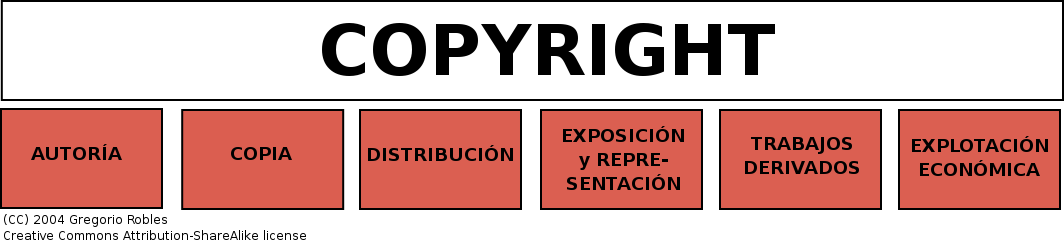
\includegraphics[width=11cm]{figs/Copyright.png}

\end{frame}

%%---------------------------------------------------------------

\begin{frame}
\frametitle{Public Domain: No rights reserved}

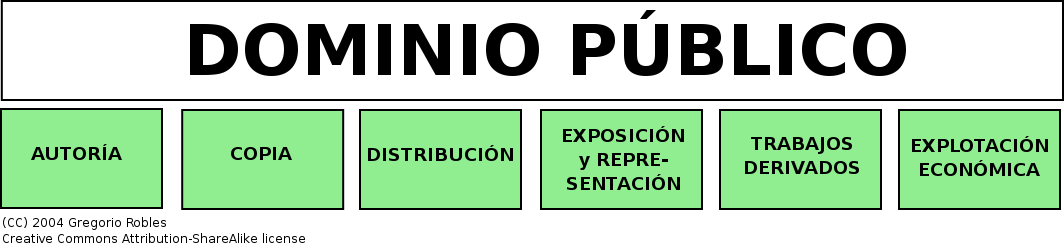
\includegraphics[width=11cm]{figs/DominioPublico.png}

\end{frame}

%%---------------------------------------------------------------

\begin{frame}
\frametitle{Creative Commons: Some rights reserved}

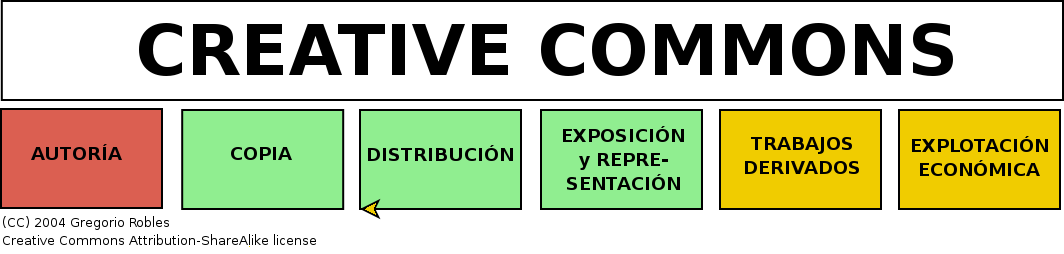
\includegraphics[width=11cm]{figs/CreativeCommons.png}

\end{frame}


%%%%%%%%%%%%%%%%%%%%%%%%%%%%%%%%%%%%%%%%%%%%%%%%%%%%%%%%%%%%%%%%%%%%%%%
\begin{frame}
\frametitle{Types of Creative Commons licenses (1/2)}

Mixing and matching these conditions produces six possible combinations:

\begin{block}{CC Licenses}
\begin{enumerate}
\item Attribution (by)
\item Attribution + Non commercial (by-nc)
\item Attribution + No Derivate Works (by-nd)
\item Attribution + share alike (by-sa)
\item Attribution + Non commercial + No Derivate Works (by-nc-nd)
\item Attribution + Non commercial + share alike (by-nc-sa)
\end{enumerate}                                                 
\end{block}
\end{frame}


%%%%%%%%%%%%%%%%%%%%%%%%%%%%%%%%%%%%%%%%%%%%%%%%%%%%%%%%%%%%%%%%%%%%%%%
\begin{frame}
\frametitle{Types of Creative Commons licenses (2/2)}

``Special'' CC licenses:
\begin{itemize}
\item Public Domain Dedication (and CC0)
\item \alert{Founder's Copyright:} the work is released into PD after 14 or 28 years.
\item \alert{Sampling Plus:} parts of the work can be copied and modified for any purpose. The entire work can be copied for non-commercial purposes.
\item \alert{Noncommercial Sampling Plus:} the whole work or parts of the work can be copied and modified for noncommercial purposes. 
\end{itemize}                                                 

Retired licenses: Developing Nations, Sampling.

\end{frame}

%%%%%%%%%%%%%%%%%%%%%%%%%%%%%%%%%%%%%%%%%%%%%%%%%%%%%%%%%%%%%%%%%%%%%%%
\begin{frame}
\frametitle{Creative Commons and software licenses}

\begin{itemize}
\item CC Licenses weren't designed for use with software: don't make mention of source or object code.
\item CC recommends to use available licenses from the free/open source software world.
\item CC has ``wrapped'' some free software/open source licenses (BSD, GPL and LGPL) with a human-readable ``Commons Deed'' and machine-readable metadata (``three-layer packaging'').
\item It is important to note that CC has not altered these software licenses in any way.
\item GPL and LGPL includes a Portuguese translation (job made for Brazilian government).
\end{itemize}                                                 

\end{frame}


%%%%%%%%%%%%%%%%%%%%%%%%%%%%%%%%%%%%%%%%%%%%%%%%%%%%%%%%%%%%%%%%%%%%%%%
\begin{frame}
\frametitle{Projects with Creative Commons licenses}

\begin{itemize}
\item \alert{Wikipedia} (cc-by-sa, since June 2009)
\item \alert{Wikia} (cc-by-sa, since June 2009). A free web hosting service for wikis
\item \alert{Citizendium} (cc-by-sa). Wiki-based Encyclopedia.
\item \alert{knol} (mostly, cc-by-sa or cc-by-nc-sa). A Google project that aims to include user-written articles on a range of topics
\item \alert{Arduino} (cc-by-sa). A single-board microcontroller and a software suite for programming it. 
\item \alert{NINJAM} (cc-by-sa). A mechanism for exchanging audio data across the internet.
\end{itemize}                                                 

\end{frame}

%%---------------------------------------------------------------


%%%%%%%%%%%%%%%%%%%%%%%%%%%%%%%%%%%%%%%%%%%%%%%%%%%%%%%%%%%%%%%%%%%%%%%
\begin{frame}
\frametitle{Use of Creative Commons licenses}

All CC licenses contain a \alert{three-layer user interface} (for humans, lawyers and machines):
\begin{itemize}
\item \alert{Commons Deed:} It is a summary, human-readable, of the license with the relevant icons.
\item \alert{Legal Code:} The complete legal code in which the chosen license is based.
\item \alert{Digital Code.} The digital code, a machine-readable version that helps search engines and other applications identify the work by its terms of use.
\end{itemize}                                                 

\end{frame}

%%---------------------------------------------------------------

\begin{frame}
\frametitle{The Attribution license}

With this license, you reserve only moral rights:

\begin{itemize}
\item Attribution of your work.
\end{itemize}

There are not restrictions in commercial use or derivative works.

This license is the nearest to a FLOSS permissive license. 

\end{frame}


%%---------------------------------------------------------------

\begin{frame}
\frametitle{The Attribution-ShareAlike license}

With this license, you reserve two rights:

\begin{itemize}
\item Attribution of your work.
\item Any derived work must be licensed under same license.
\end{itemize}

This license is the nearest to a copyleft license. 

\end{frame}

%%---------------------------------------------------------------

\begin{frame}
\frametitle{CC Zero license}


\begin{itemize}
\item Created in 2009.
\item CC0 is the ``no rights reserved'' option (like a PD dedication).
\item Anyone can then use the work in any way and for any purpose
\item Public Domain legally robust way: universal applicability, intended for use world-wide by anyone.
\item If the waiver isn't effective for any reason, then CC0 acts as a license from the affirmer granting the public an unconditional, irrevocable, non exclusive, royalty free license to use the work for any purpose. 
\end{itemize}


\end{frame}

%%---------------------------------------------------------------

\begin{frame}
\frametitle{CC Zero (CC0) -- No Copyright}

\begin{block}{CC0 Public Domain Dedication}
``The person who associated a work with this deed has dedicated the work to the public domain by waiving all of his or her rights to the work worldwide under copyright law, including all related and neighboring rights, to the extent allowed by law.''
\end{block}

\medskip

\small
CC0 rights granted: ``\alert{You can copy, modify, distribute and perform the work, even for commercial purposes, all without asking permission.}''

\end{frame}

%%---------------------------------------------------------------

\begin{frame}
\frametitle{CC Zero (CC0) -- No Copyright}

\begin{center}

\includegraphics[width=8cm]{figs/cc0.png}
\end{center}


\end{frame}

%%%%%%%%%%%%%%%%%%%%%%%%%%%%%%%%%%%%%%%%%%%%%%%%%%%%%%%%%%%%%%%%%%%%%%%
\begin{frame}
\frametitle{CC NonCommercial Share-alike (CC-nc-sa)}

Is it a free license?
\pause

\begin{itemize}
\item CC-nc-sa is \alert{NOT} a free license.
\end{itemize}                                                 

\pause

Is it a copyleft license?
\pause

\begin{itemize}
\item NonCommercial Share-alike is \alert{NOT} a copyleft license: copyleft rebuilds and protects the rights that restrictive copyright removes.
\item \alert Rights, no \textit{some} rights.
\end{itemize}                                                 

\end{frame}



%%%%%%%%%%%%%%%%%%%%%%%%%%%%%%%%%%%%%%%%%%%%%%%%%%%%%%%%%%%%%%%%%%%%%%%
\begin{frame}
\frametitle{¿What does it mean non-commercial?}

\begin{block}{Noncommercial clause}
\small

You may not exercise any of the rights granted to You [...] in any manner that is primarily intended for or directed toward commercial advantage or private monetary compensation. 



\end{block}

\end{frame}


%%%%%%%%%%%%%%%%%%%%%%%%%%%%%%%%%%%%%%%%%%%%%%%%%%%%%%%%%%%%%%%%%%%%%%%

\begin{frame}
\frametitle{The ``non-commercial'' clause (1/3)}

\begin{itemize}
\item It is frequently used, particularly in blogs and social sites, and it is now being adopted by some institutions.
\item They are believed to protect the work against abusive use and opportunists (reselling or commercial exploitation by corporations, etc.).
\item It is sometimes supported by alleging that protects investment (though some studies have challenged this view, since it restricts distribution).
\end{itemize}                                                 

\end{frame}

%%%%%%%%%%%%%%%%%%%%%%%%%%%%%%%%%%%%%%%%%%%%%%%%%%%%%%%%%%%%%%%%%%%%%%%

\begin{frame}
\frametitle{The ``non-commercial'' clause (2/3)}

It raises evil side effects: 
\begin{itemize}
\item This clause does not distinguish between indirect commercial uses, self-funded projects, etc.
\item It brings uncertainty about what is a commercial activity: when in doubt you might decide not to use it to avoid demands or consulting lawyers... 
\item Incompatibility with libre projects (i.e. Wikipedia).
\item Causing confusion about  the ``free'' concept: it promotes another kind of opportunism, by using viral marketing to create the impression that a work is free but not truly releasing it as a libre product.
\end{itemize}                                                 

\end{frame}

%%%%%%%%%%%%%%%%%%%%%%%%%%%%%%%%%%%%%%%%%%%%%%%%%%%%%%%%%%%%%%%%%%%%%%%

\begin{frame}
\frametitle{The ``non-commercial'' clause (3/3)}

\begin{itemize}
\item The author's right to decide the terms in which he shares his work is not at stake here.
\item What it is rejected is the confusion and the subterfuge of presenting a work as a free product when it is not true.
\item Use any license you like, but also use concepts with accuracy: do not label as \textit{free/libre} or \textit{copyleft} what it is not. Confusion damages free culture and benefit opportunists.
\end{itemize}
\end{frame}

%%%%%%%%%%%%%%%%%%%%%%%%%%%%%%%%%%%%%%%%%%%%%%%%%%%%%%%%%%%%%%%%%%%%%%%

\begin{frame}
\frametitle{Exercise: Choose a license}

\begin{itemize}
\item Choose a CC License for your blog
\end{itemize}
\end{frame}



%%%%%%%%%%%%%%%%%%%%%%%%%%%%%%%%%%%%%%%%%%%%%%%%%%%%%%%%%%%%%%%%%%%%%%%

\begin{frame}
\begin{center}
\huge{Debian Guidelines and Creative Commons Licenses}
\end{center}

\end{frame}


%%---------------------------------------------------------------

\begin{frame}
\frametitle{Debian-legal enters the arena}

After the popularization of CC, Debian-legal warned of
Attribution provisions. The causes were:

\begin{itemize}
\item A work under Attribution can be in fact, NoDerivs 
\item Downstream users remove an author's credit upon request from the author.
\item Inaccurate or excessive authorship credits.
\item Problems with Anti-DRM provisions (which could restrict private redistribution to some extent).
\item Trademark restrictions.
\item Attribution[-ShareAlike] 2.x is NOT compatible with DFSG. 
\item Efforts to fix these problems in the new version 3.0 licenses.

\end{itemize}


\end{frame}



%%---------------------------------------------------------------

\begin{frame}
\frametitle{CC Attribution Problems (I)}

\begin{itemize}
\item Licensor/Original Author can request removal of him/her references in derived works.
\item However the author name must be included in derivative works ``if supplied'' (Attribution)
\end{itemize}

It's unclear if creator of derivative works can comply with a requirement of removing references and requirement of give attribution. Then, a request to remove references can make impossible to comply with Attribution; so it may not be possible to make derivative/collective works under this license (DFSG 3 \& 1 incompatible). {\bf The work is not free?}

\end{frame}

%%---------------------------------------------------------------

\begin{frame}
\frametitle{CC Attribution Problems (II): Authorship credits}

\begin{itemize}
\item Requirements for crediting Licensor for his/her work: it's ambiguous
\item So, we need the most pessimistic interpretation:
\begin{itemize}
\item Required attribution for the licensor everywhere that authorship credit is given.
\end{itemize}
% \item Excessive/Inaccurate authorship credits: DFSG 1 \& 3 incompatible.
\end{itemize}
Example 1: {\it If a work is a collection of essays by different authors, with authorship credit given in the chapter titles, the Licensor's name would have to be listed for each chapter title, even if they did not contribute to it.}\\
Example 2: {\it If Alice writes her autobiography, and includes lyrics from Bob's song in one chapter, she must give him credit for the entire work: ``The Autobiography of Alice, by Alice and Bob'', or even ``The Autobiography of Alice and Bob.''}
\end{frame}

%%---------------------------------------------------------------

\begin{frame}
\frametitle{CC Attribution Problems (III)}

\begin{itemize}
\item Anti-DRM Clause: Distribution with measures to control access is not compatible with DFSG 1.
\end{itemize}

Example 1: Private distribution of work might be forbidden.\\
Example 2: Distribution in a server with control access (i.e. firewall) might be forbidden.
\end{frame}

%%---------------------------------------------------------------

\begin{frame}
\frametitle{CC Attribution Problems (IV)}

\begin{itemize}
\item Web page says: Using CC trademark or logos is strictly prohibited when it's used for other than indicating the work is licensed under CC.
\item Although CC Trademark not appears to be part of the CC licenses, this is only warned in ``source code'' of CC web page.
\item Interpretation: This can prevent redistribution, modification ...
\end{itemize}

\end{frame}

%%---------------------------------------------------------------

\begin{frame}
\frametitle{CC NoDerivs clause problems}

\LARGE{Obviously, NoDerivs licenses are not compatible with Four Freedoms (nor DFSG)}

\end{frame}

%%---------------------------------------------------------------

\begin{frame}
\frametitle{CC NonCommercial clause problems}

\LARGE{Obviously, NonCommercial licenses are not compatible with Four Freedoms (nor DFSG)}

\end{frame}

%%---------------------------------------------------------------


\begin{frame}
\frametitle{Debian recommendations to authors}

\begin{itemize}
\item All software licensed under CC 2.x is NOT compatible with DFSG. 
\item CC 3.x has fixed several of these problems.
\item Software licensed under NonCommercial/NoDerivs can't be named ``Free Software''.
\item Authors who wish to use Attribution must use other licenses as BSD.
\item Authors who wish to use Attribution-ShareAlike must use other licenses as GFDL.
\end{itemize}

\end{frame}


%%---------------------------------------------------------------
%%%%%%%%%%%%%%%%%%%%%%%%%%%%%%%%%%%%%%%%%%%%%%%%%%%%%%%%%%%%%%%%%%%%%%%
% \section{References}
%%%%%%%%%%%%%%%%%%%%%%%%%%%%%%%%%%%%%%%%%%%%%%%%%%%%%%%%%%%%%%%%%%%%%%%

% \begin{frame}
% \frametitle{References}

% \begin{itemize}
% \item \textsc{Van Lindberg}, \textit{Intellectual Property and Open Source}, O'Reilly, July 2008.
% \item \textsc{Malcolm Bain} et al. \textit{Aspectos legales y de explotación del software libre}, UOC, February 2007. \\
% \url{http://ocw.uoc.edu/informatica-tecnologia-y-multimedia/aspectos-legales-y-de-explotacion-del-software-libre/materiales/}
% \item \textsc{Lawrence Rose}, \textit{Open Source Licensing}, Prentice Hall, July 2004 
% \end{itemize}

% \end{frame}


%%%%%%%%%%%%%%%%%%%%%%%%%%%%%%%%%%%%%%%%%%%%%%%%%%%%%%%%%%%%%%%%%%%%%%%


%%---------------------------------------------------------------


%\begin{frame}
%\frametitle{Exercise: Analyze a software public license}

%Search on the web the EUPL License (versions 1.0 and 1.1). Read it in the language of your choice.

%\begin{itemize}
%\item What kind of license is? (Non-free/permissive/recíprocal...)
%\item How does it solve incompatibility with copyleft licenses?
%\item Analyse carefully section 13 of both versions (1.0 and 1.1). What has it been changed? What do you think it was due this change?
%\item Is it applicable outside the EU? What is the geographic scope of the license?
%\item Does it have anti-patent defense? If yes, how is it implemented? (Quoting the passage). How does it work?
%\item Has it Affero clause? Where?
%\end{itemize}

%\end{frame}


% %% lic_prac.tex
%%
%% Presentation of the course ``Legal Issues'' of the Official Master on Libre Software (URJC)
%% http://master.libresoft.es
%%


%%---------------------------------------------------------------------
%%---------------------------------------------------------------------

\begin{frame}
  \frametitle{Course Contents}

  \begin{itemize}
    \item Lesson 0: Presentation of the Course
    \item Lesson 1: Intellectual Property: basic concepts and legal framework
    \item Lesson 2: Legal Aspects of Libre Software
    \item Lesson 3: Libre software licenses
    \item Lesson 4: Free licenses for other intellectual works
    \item \alert{Lesson 5: Case studies}
  \end{itemize}

\end{frame}

%%%%%%%%%%%%%%%%%%%%%%%%%%%%%%%%%%%%%%%%%%%%%%%%%%%%%%%%%%%%%%%%%%%%%%%
\section{Lesson V: Practical Issues. Case studies}
%%%%%%%%%%%%%%%%%%%%%%%%%%%%%%%%%%%%%%%%%%%%%%%%%%%%%%%%%%%%%%%%%%%%%%%

%%%%%%%%%%%%%%%%%%%%%%%%%%%%%%%%%%%%%%%%%%%%%%%%%%%%%%%%%%%%%%%%%%%%%%%

\begin{frame}
\frametitle{Choosing a free license: previous criteria}

\begin{itemize}
\item Each project has its own goals and criteria related to licensing issues.
\item The main criteria of differentiation is existence (or not) of \alert{reciprocity pacts}.
\item Other copyleft licenses have a limited effect, which applies only to the work (or component) original (weak copyleft). 
\item Dual licensing policies.

\end{itemize}

\end{frame}

%%%%%%%%%%%%%%%%%%%%%%%%%%%%%%%%%%%%%%%%%%%%%%%%%%%%%%%%%%%%%%%%%%%%%%%

\begin{frame}
\frametitle{Choosing a free license: When?}

\begin{itemize}
\item When we want to guarantee some basic freedoms, common to all free software.
\item When we want a work achieves the highest use and dissemination (permissive licenses).
\item When we want to maintain control over the evolution of the program (copyleft licenses).
\item When we impose certain conditions or restrictions (the recognition of authorship, lack of liability, extra warranties, trademarks, etc.)
\end{itemize}

\end{frame}

%%%%%%%%%%%%%%%%%%%%%%%%%%%%%%%%%%%%%%%%%%%%%%%%%%%%%%%%%%%%%%%%%%%%%%%

\begin{frame}
\frametitle{How to know when a software license is free?}

\begin{center}
\includegraphics[width=6.5cm]{figs/chart.jpg}
\end{center}

\end{frame}

%%%%%%%%%%%%%%%%%%%%%%%%%%%%%%%%%%%%%%%%%%%%%%%%%%%%%%%%%%%%%%%%%%%%%%%

\begin{frame}
\frametitle{How to know when a software license is free?}

\begin{center}
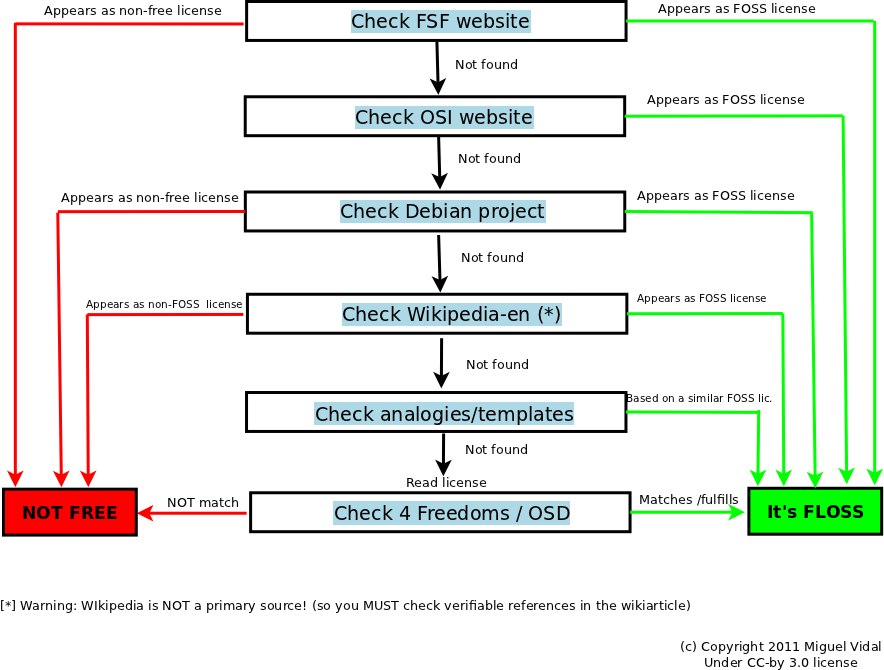
\includegraphics[width=10cm]{figs/flowchart-licenses.png}
\end{center}

\end{frame}


%%%%%%%%%%%%%%%%%%%%%%%%%%%%%%%%%%%%%%%%%%%%%%%%%%%%%%%%%%%%%%%%%%%%%%%

\begin{frame}
\frametitle{Choosing a free license: Cases}

\begin{itemize}
\item Do I want to allow privatization of derivative works?
\pause
\item Do I want developers return their modifications to the community, or me as original author, in particular?
\pause
\item Do I want to allow licensees to merge or link their program with mine?
\pause
\item Do I want widespread coverage and/or try to establish a standard?
\pause
\item Should my program run with one in particular? Have it any restrictions?
\pause
\item Is there risk that someone requiring a patent license over program?
\end{itemize}


\end{frame}

%%%%%%%%%%%%%%%%%%%%%%%%%%%%%%%%%%%%%%%%%%%%%%%%%%%%%%%%%%%%%%%%%%%%%%%

\begin{frame}
\frametitle{Quick Reference For Choosing a Free Software License}

\begin{center}
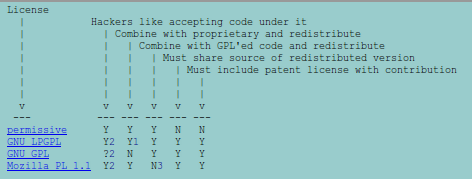
\includegraphics[width=11.5cm]{figs/licenses_quick_reference.png}
\end{center}

\end{frame}

%%%%%%%%%%%%%%%%%%%%%%%%%%%%%%%%%%%%%%%%%%%%%%%%%%%%%%%%%%%%%%%%%%%%%%%

\begin{frame}
\frametitle{Exercise: Find mistakes}

\begin{center}
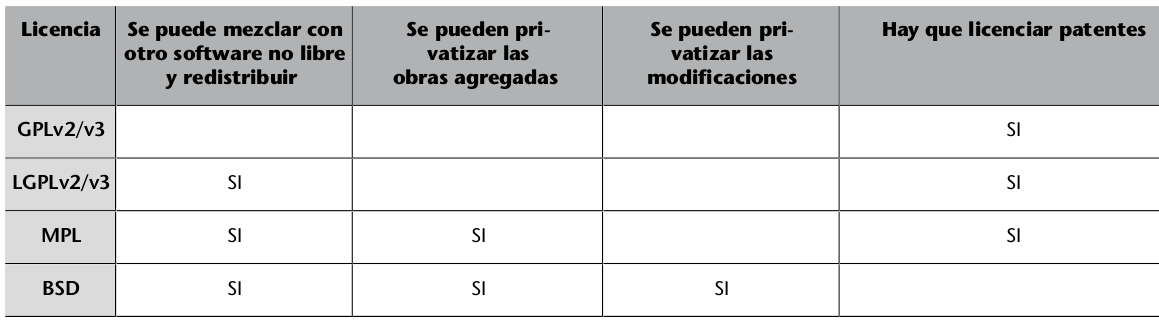
\includegraphics[width=11.5cm]{figs/tabla_licencias.png}
\end{center}

\end{frame}

%%%%%%%%%%%%%%%%%%%%%%%%%%%%%%%%%%%%%%%%%%%%%%%%%%%%%%%%%%%%%%%%%%%%%%%

\begin{frame}
\frametitle{Conventional Matrix}

\begin{center}
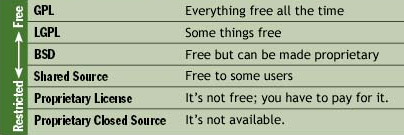
\includegraphics[width=11.5cm]{figs/conventional_matrix.png}
\end{center}

\end{frame}

%%%%%%%%%%%%%%%%%%%%%%%%%%%%%%%%%%%%%%%%%%%%%%%%%%%%%%%%%%%%%%%%%%%%%%%

\begin{frame}
\frametitle{Matrix Including Developer's Choice}

\begin{center}
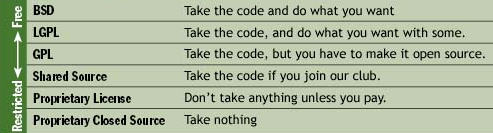
\includegraphics[width=11.5cm]{figs/matrix_developers_choice.png}
\end{center}

\end{frame}


%%%%%%%%%%%%%%%%%%%%%%%%%%%%%%%%%%%%%%%%%%%%%%%%%%%%%%%%%%%%%%%%%%%%%%%

\begin{frame}
\frametitle{Remarks}

\begin{itemize}
\item Some members of the community refuse to accept GPL'ed source code into their projects.
\item Other members of the community strongly prefer GPL'ed source code over other licenses.
\item Nobody refuses to accept code under permissive licenses such as BSD, X11, MIT... 
\end{itemize}

\end{frame}

%%%%%%%%%%%%%%%%%%%%%%%%%%%%%%%%%%%%%%%%%%%%%%%%%%%%%%%%%%%%%%%%%%%%%%%

\begin{frame}
\frametitle{Remarks (2)}

\begin{itemize}
\item Almost nobody refuses to accept LGPL'ed code, except the Apache Foundation, saying that they think it would impose LGPL requirement upon the proprietary code (when they are linked via the Java class-loading mechanism).
\item The FSF disagrees with this statement, asserting that such linking falls under section 6 of the LGPLv2 (linking exception).
\end{itemize}

\end{frame}

%%%%%%%%%%%%%%%%%%%%%%%%%%%%%%%%%%%%%%%%%%%%%%%%%%%%%%%%%%%%%%%%%%%%%%%

\begin{frame}
\frametitle{Remarks (and 3)}

\begin{itemize}
\item MPL 1.1 can be specifically amended to allow combining with GPL (section 13).
\item You should also get your employer (if you work as a programmer) or school, to sign a ``copyright disclaimer'' for the program, if necessary. 
\end{itemize}

\end{frame}


%%%%%%%%%%%%%%%%%%%%%%%%%%%%%%%%%%%%%%%%%%%%%%%%%%%%%%%%%%%%%%%%%%%%%%%

\begin{frame}
\frametitle{Applying a free license}


\begin{itemize}
\item \texttt{LICENSE} or \texttt{COPYING} file.
\item Copyright and license summary at the beginning of each source file.
\item It should have at least the ``copyright'' notice and a link to the full version of the license.
\item Also add information on how to contact you by electronic and paper mail.
\item If the program is interactive (terminal), make it output a short copyright notice 
when it starts in an interactive mode.
\item If it has a GUI, a menu can include copyright notice (or even the full license).
\end{itemize}

\end{frame}

%%%%%%%%%%%%%%%%%%%%%%%%%%%%%%%%%%%%%%%%%%%%%%%%%%%%%%%%%%%%%%%%%%%%%%%

\begin{frame}
\frametitle{Example: How to Apply the GPL to Your Work}

\footnotesize

\texttt{<one line with program's name and a brief idea of what it does.>} \\
\texttt{Copyright (C) <year>  <name of author>}

\medskip

\texttt{This program is free software: you can redistribute it and/or modify
    it under the terms of the GNU General Public License as published by
    the Free Software Foundation, either version 3 of the License, or
    (at your option) any later version.}

\medskip

\texttt{This program is distributed in the hope that it will be useful,
    but WITHOUT ANY WARRANTY; without even the implied warranty of
    MERCHANTABILITY or FITNESS FOR A PARTICULAR PURPOSE.  See the
    GNU General Public License for more details.}

\medskip

\texttt{You should have received a copy of the GNU General Public License
    along with this program.  If not, see <http://www.gnu.org/licenses/>.}


\end{frame}

%%%%%%%%%%%%%%%%%%%%%%%%%%%%%%%%%%%%%%%%%%%%%%%%%%%%%%%%%%%%%%%%%%%%%%%

\begin{frame}
\frametitle{Example: How to Apply the Apache License to Your Work}

\footnotesize

\texttt{Copyright [yyyy] [name of copyright owner]}

\medskip

\texttt{Licensed under the Apache License, Version 2.0 (the ``License'');
   you may not use this file except in compliance with the License.
   You may obtain a copy of the License at http://www.apache.org/licenses/LICENSE-2.0}

\medskip

\texttt{Unless required by applicable law or agreed to in writing, software
   distributed under the License is distributed on an ``AS IS'' BASIS,
   WITHOUT WARRANTIES OR CONDITIONS OF ANY KIND, either express or implied.
   See the License for the specific language governing permissions and
   limitations under the License.}


\end{frame}

%%%%%%%%%%%%%%%%%%%%%%%%%%%%%%%%%%%%%%%%%%%%%%%%%%%%%%%%%%%%%%%%%%%%%%%

\begin{frame}
\frametitle{Example: How to Apply the ISC License to Your Work (1)}

\begin{itemize}
\item Below is an example license to be used for new code in OpenBSD,
modeled after the ISC license.
\item It is important to specify the year of the copyright.  Additional years
should be separated by a comma, e.g.
    Copyright (c) 2003, 2004
\item If you add extra text to the body of the license, be careful not to
add further restrictions.
\end{itemize}

\end{frame}

%%%%%%%%%%%%%%%%%%%%%%%%%%%%%%%%%%%%%%%%%%%%%%%%%%%%%%%%%%%%%%%%%%%%%%%

\begin{frame}
% \frametitle{Example: How to Apply the ISC License to Your Work (and 2)}

\begin{block}{Example: How to Apply the ISC License to Your Work}
\footnotesize
/* \\
 * Copyright (c) CCYY YOUR NAME HERE $<$user@your.dom.ain$>$ \\
 * \\
 * Permission to use, copy, modify, and distribute this software \\
 * for any purpose with or without fee is hereby granted, provided \\
 * that the above copyright notice and this permission notice appear \\
 * in all copies. \\
 * \\
 * THE SOFTWARE IS PROVIDED "AS IS" AND THE AUTHOR DISCLAIMS \\
 * ALL WARRANTIES WITH REGARD TO THIS SOFTWARE INCLUDING \\
 * ALL IMPLIED WARRANTIES OF MERCHANTABILITY AND FITNESS. \\
 * IN NO EVENT SHALL THE AUTHOR BE LIABLE FOR ANY SPECIAL, \\
 * DIRECT, INDIRECT, OR CONSEQUENTIAL DAMAGES OR ANY \\
 * DAMAGES WHATSOEVER RESULTING FROM LOSS OF USE, DATA OR \\
 * PROFITS, WHETHER IN AN ACTION OF CONTRACT, NEGLIGENCE OR \\
 * OTHER TORTIOUS ACTION, ARISING OUT OF OR IN CONNECTION \\
 * WITH THE USE OR PERFORMANCE OF THIS SOFTWARE. \\
 */
\end{block}

\end{frame}



%%%%%%%%%%%%%%%%%%%%%%%%%%%%%%%%%%%%%%%%%%%%%%%%%%%%%%%%%%%%%%%%%%%%%%%
\begin{frame}
\frametitle{Dual-licensing}

Distribute software under two different sets of terms and conditions. Motivations:

\begin{itemize}
\item License compatibility (Perl, Mozilla/Firefox, MySQL).
\item Market segregation based business models (MySQL Enterprise)
\item Allows the holder to offer customisations, early releases, generate other derivative works or grant rights to third parties to redistribute proprietary versions.
\end{itemize}

                                                 
\end{frame}


%%%%%%%%%%%%%%%%%%%%%%%%%%%%%%%%%%%%%%%%%%%%%%%%%%%%%%%%%%%%%%%%%%%%%%%

\begin{frame}
\frametitle{Compatibility}

\begin{itemize}
\item Two licenses are incompatible if it is not possible combining both works in compliance with the terms of  both licenses at the same time. 
\item It affects to distribution, not the use. 
\item If two licenses are free does, it doesn't imply are compatible. 
\item Copyleft licenses are mutually incompatible, unless compatibility is declared explicitly. 
\item Support for `` linking'': even if not allowed mix or integrate software with different licenses, maybe it can be linked. 
\end{itemize}

\end{frame}

%%%%%%%%%%%%%%%%%%%%%%%%%%%%%%%%%%%%%%%%%%%%%%%%%%%%%%%%%%%%%%%%%%%%%%%

\begin{frame}
\frametitle{Forking (1)}

\begin{itemize}
\item A piece of software is modified and developed separately by another team development, and distributed under a different name, and maybe other
license.
\item The forks can be possible \alert{only} with free/open source software.
\item The GPL software has tendency to avoid forking (we must keep the original license).
\item The BSD-style licenses are forked easily.
\end{itemize}

\end{frame}

%%%%%%%%%%%%%%%%%%%%%%%%%%%%%%%%%%%%%%%%%%%%%%%%%%%%%%%%%%%%%%%%%%%%%%%

\begin{frame}
\frametitle{Forking (and 2)}

\begin{itemize}
\item Forking is considered a bad thing (waste efforts, bitter disputes...).
\item But there are successful cases: XOrg/XFree86, 386BSD, OpenBSD, Gnu-Emacs/XEmacs, changes of license (GForge, OpenSSH).
\end{itemize}

\end{frame}


%%%%%%%%%%%%%%%%%%%%%%%%%%%%%%%%%%%%%%%%%%%%%%%%%%%%%%%%%%%%%%%%%%%%%%%

\begin{frame}
\frametitle{Licenses and warranty}

\begin{itemize}
\item Warranty disclaimers and limitation of liability clauses are common in software.
\item There are legal doubts about the effectiveness of these clauses: \alert{would not apply to consumers}.
\item This clauses are valid when there is \alert{no commercial service}.
\item The proprietary licenses using similar terms: is a myth to accept greater responsibility.
\item It must be considered legal guarantees that apply to both open source and proprietary software.
\item The free licenses allow (sometimes) to add extra warranty clauses.
\end{itemize}


\end{frame}

%%%%%%%%%%%%%%%%%%%%%%%%%%%%%%%%%%%%%%%%%%%%%%%%%%%%%%%%%%%%%%%%%%%%%%%

\begin{frame}
\frametitle{Exercise: Case study}


\begin{itemize}
\item Case study: Apache License v2 and GPL (v2 and v3)  (in)compatibility.
\item Moodle exercise.
\end{itemize}

\end{frame}


%%%%%%%%%%%%%%%%%%%%%%%%%%%%%%%%%%%%%%%%%%%%%%%%%%%%%%%%%%%%%%%%%%%%%%%

\begin{frame}
\frametitle{Exercise: Case study}


\begin{itemize}
\item Case study: GPL and CDDL incompatibility. 
\item Moodle exercise.
\end{itemize}

\end{frame}


%%%%%%%%%%%%%%%%%%%%%%%%%%%%%%%%%%%%%%%%%%%%%%%%%%%%%%%%%%%%%%%%%%%%%%%

\begin{frame}
\frametitle{Exercise: Case study}


\begin{itemize}
\item Case study: The EUPL
\item Moodle Exercise 
\end{itemize}

\end{frame}


%%==================================================================
%%---------------------------------------------------------------




\end{document}
